\documentclass{book}

\usepackage{times,mathptmx}
\usepackage[pdftex]{graphicx}
\usepackage{pdflscape}

\usepackage{booktabs}
\usepackage{subcaption}
\usepackage{graphicx}
\usepackage{float}
\usepackage[section]{placeins}
\usepackage{fancyhdr}
\usepackage{enumitem}

\usepackage{tocloft}
\usepackage[nottoc,notlof,notlot]{tocbibind} % Put the bibliography and index in the ToC

\pagestyle{fancy}
\rhead{}
\lhead{}
\chead{Page \thepage}
\cfoot{Predecisional Draft Report}
%\renewcommand{\headrulewidth}{0.4pt}
\renewcommand{\footrulewidth}{0.4pt}

\usepackage{color}
\usepackage{amsmath}
\usepackage{siunitx}
\usepackage{multirow}
\definecolor{linknavy}{rgb}{0,0,0.50196}
\definecolor{linkred}{rgb}{1,0,0}
\definecolor{linkblue}{rgb}{0,0,1}

\usepackage{xr-hyper}
\usepackage[pdftex,
        colorlinks=true,
        urlcolor=linkblue,     % \href{...}{...} external (URL)
        citecolor=linkred,     % citation number colors
        linkcolor=linknavy,    % \ref{...} and \pageref{...}
        pdfproducer={pdflatex},
        pagebackref,
        pdfpagemode=UseNone,
        bookmarksopen=true,
        plainpages=false,
        verbose]{hyperref}

\setlength{\textwidth}{6.5in}
\setlength{\textheight}{9.0in}
\setlength{\topmargin}{0.in}
\setlength{\headheight}{0.in}
\setlength{\headsep}{0.25in}
\setlength{\parindent}{0.25in}
\setlength{\oddsidemargin}{0.0in}
\setlength{\evensidemargin}{0.0in}




\begin{document}

\bibliographystyle{unsrt}
\thispagestyle{empty}


\vspace*{0.75in}

\begin{center}
\begin{Large}
{\bf Preliminary Summary of Experimental Measurements} \\
\end{Large}
\hspace{1in} \\
\end{center}

\begin{center}
\begin{large}
Predecisional Draft Report\\
Submitted to the MaCFP-4 Condensed Phase Workshop \\
Version 1.0 -- Released: March 30, 2026\\
\end{large}
\hspace{2in} \\
\end{center}

\begin{figure}[h]
  \centering
  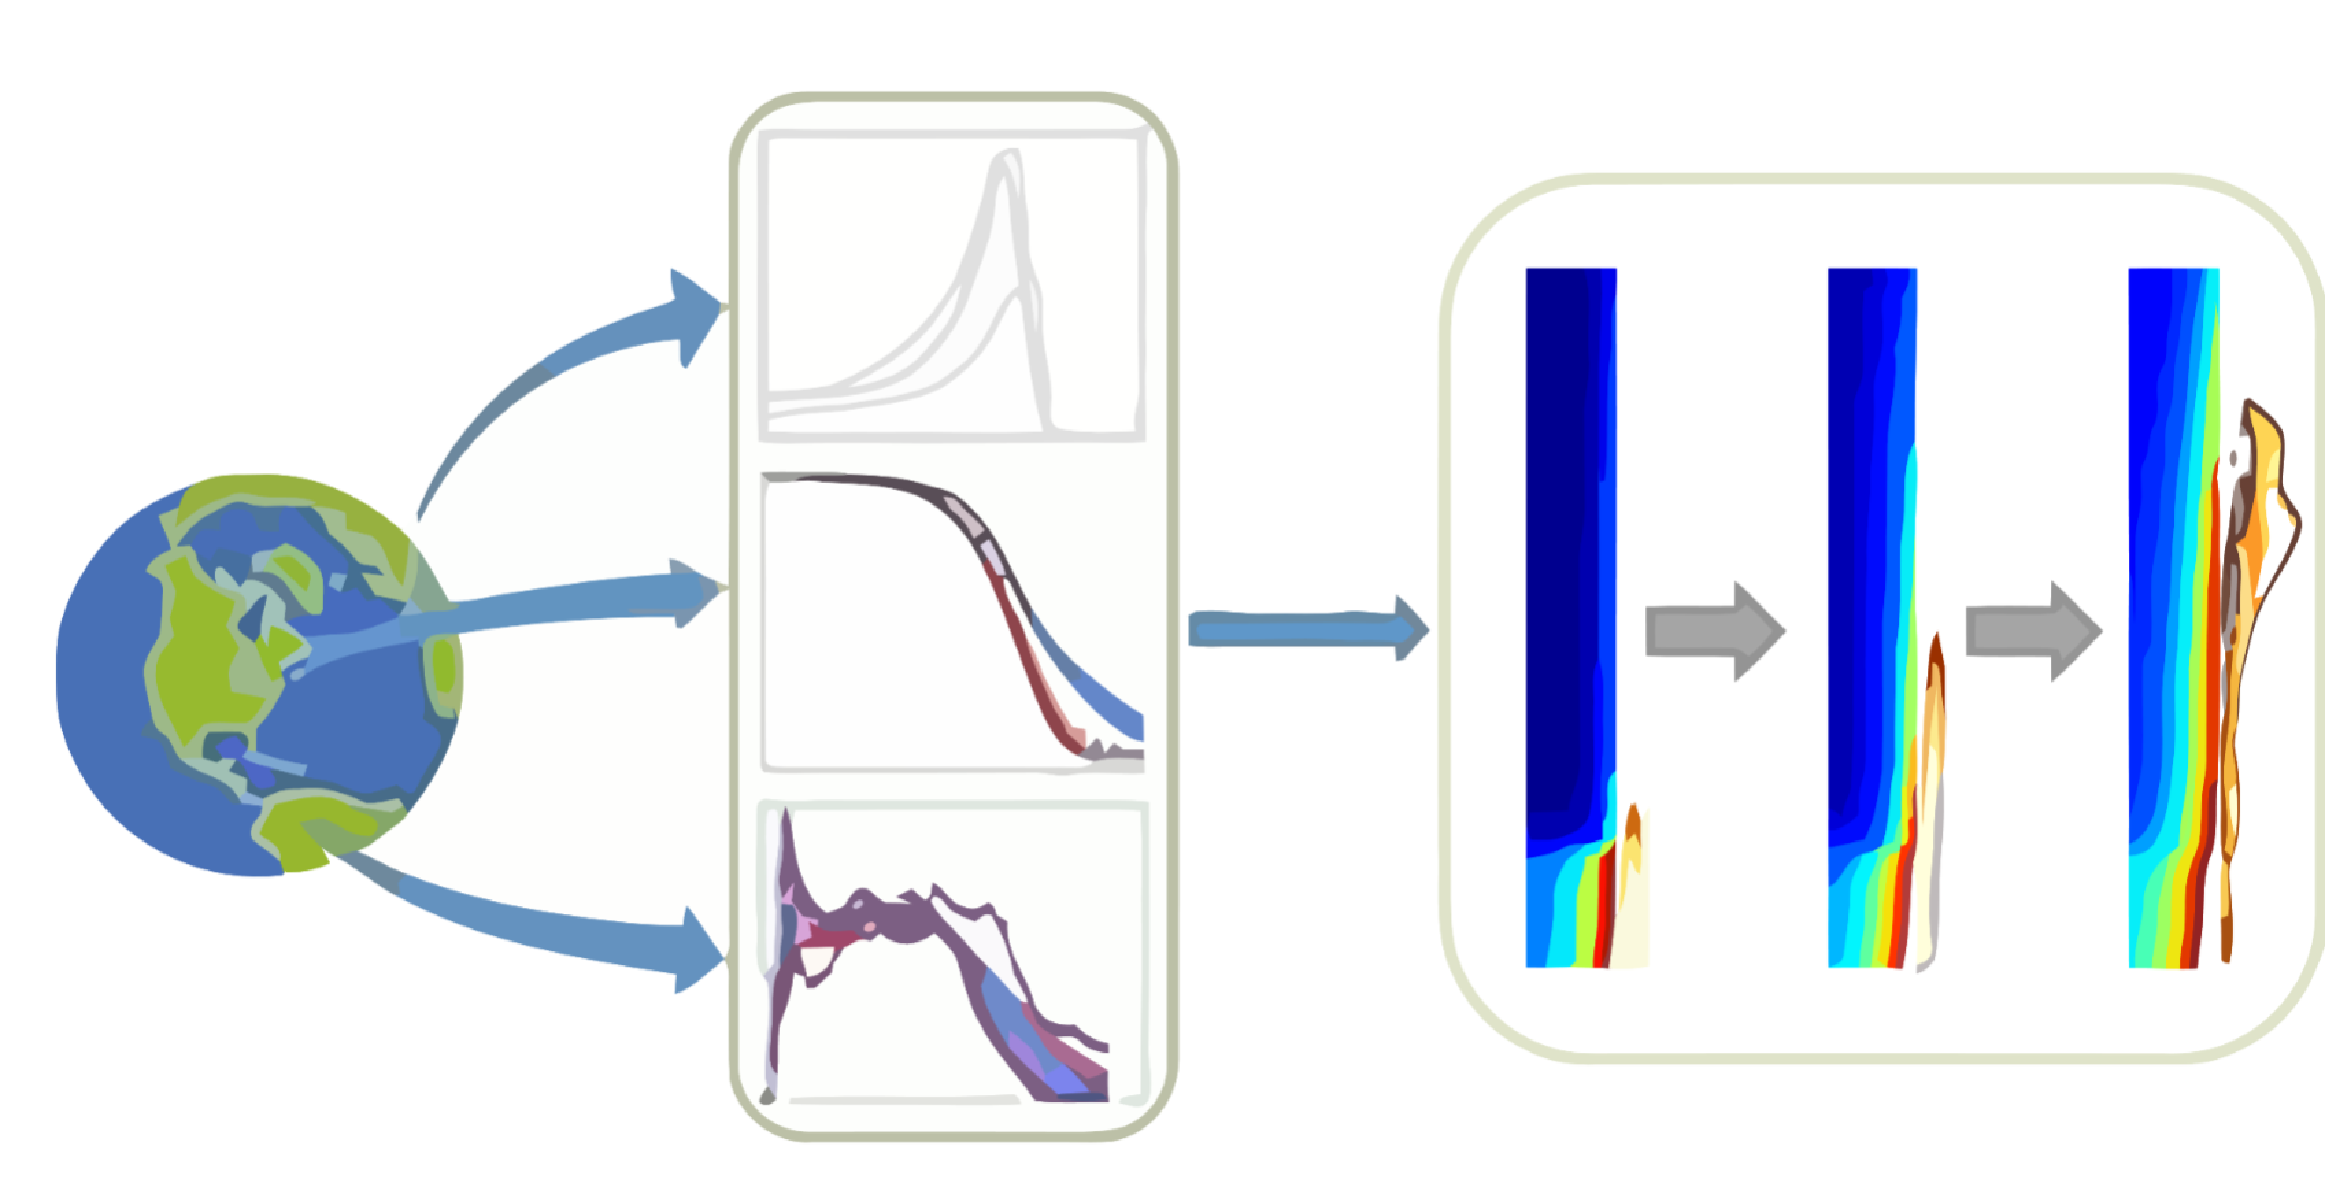
\includegraphics[width=6in]{../FIGURES/MaCFP_Logo}
  \label{Cover_Image}
\end{figure}

\vfill

\begin{minipage}{0.25\textwidth}
\begin{figure}[H]

\includegraphics[width=1.5in]{../FIGURES/IAFSSLogo}
\end{figure}
\end{minipage} \hfill
\begin{minipage}{0.7\textwidth}
\begin{flushright}
%{\bf The MaCFP Condensed Phase Working Group Organizing Committee:} \\
%Benjamin Batiot (University of Poitiers, France) \\
%Morgan Bruns (Virginia Military Institute, USA) \\
%Simo Hostikka (Aalto University, Finland) \\
%Isaac Leventon (National Institute of Standards and Technology, USA) \\
%Yuji Nakamura (Toyohashi University of Technology, Japan) \\
%Pedro Reszka (Universidad Adolfo Ibáñez, Chile) \\
%Thomas Rogaume (University of Poitiers, France) \\
%Stanislav Stoliarov (University of Maryland, USA)
\textbf{ Document Prepared by:} \\
Isaac Leventon and Karen De Lannoye\\
(National Institute of Standards and Technology, NIST) \\
\textbf{Experimental Results Submitted by:}\\
Sina Bazrpash, Simo Hostikka; Aalto University. 
%Nicolas Cabaret, Bertrand Girardin; Centre d’Essais au Feu (CERIB). 
Yan Ding; China University of Geosciences. 
Lukas Arnold, Alex Belt, Tristan Hehnen; Forschungszentrum Jülich. 
Shaorun Lin, Xinyan Huang; Hong Kong Polytechnical University. 
Rodolphe Sonnier; IMT Mines Alès. 
%Konrad Wilkens; Lund University. 
Nathan Kahla, Sara McAllister; Missoula Fire Sciences Lab (MFSL). 
Ryan Greene, Karen De Lannoye, Isaac Leventon; National Institute of Standards and Technology (NIST). 
Lucie Hasalová; Technical Institute of Fire Protection in Prague (TIFP). 
Vojtech Salek; University of Chemistry and Technology in Prague (UCT)
Felix Armbrust; Technische Universität Braunschweig. 
Yuji NAKAMURA; Toyohashi University of Technology. 
Pedro Reszka; Universidad Adolfo Ibáñez (UAI). 
David Lázaro Urrutia; Universidad de Cantabria. 
Mark McKinnon; UL Fire Safety Research Institute (UL FSRI). 
Alexander Morgan; University of Dayton Research Institute (UDRI).  
Serge Bourbigot, Johan Sarazin; Université de Lille (UMET). 
Grayson Bellamy, Stanislav Stoliarov; University of Maryland (UMD). 
Marc Poisson, Benjamin Batiot, Thomas Rogaume; Université de Poitiers. 
Laura Hasburgh; USDA Forest Products Laboratory. 
%Wenxuan Wu, David Morrisset; The University of Queensland (UQ).

\end{flushright}
\end{minipage}


\newpage
\thispagestyle{empty}

\frontmatter

\chapter{Preface}
\thispagestyle{fancy}
This report has been prepared on behalf of the MaCFP Condensed Phase Working Group. It is a predecisional draft copy prepared for subject matter experts to provide critical review and to ensure the integrity of the measurement data and related analysis submitted to the MaCFP-4 Condensed Phase Workshop.

Parts of this work were prepared by the National Institute of Standards and Technology (NIST), an agency of the US government, and is not subject to copyright in the USA. Not all of the measurement data presented here has been through a formal review process. The identification of any commercial product or trade name does not imply endorsement or recommendation by NIST (or any other contributing institution). The policy of NIST is to use metric units of measurement in all its publications, and to provide statements of uncertainty for all original measurements. In this document, however, data from organizations outside NIST are shown, which may include measurements in non-metric units or measurements without uncertainty statements.



\newpage
\thispagestyle{fancy}
\tableofcontents

\mainmatter
\pagestyle{fancy}

\chapter{Introduction}
In April 2016, it was proposed that the Measurement and Computation of Fire Phenomena (MaCFP) Working Group be expanded to include a subgroup dedicated to the predictive modeling of condensed phase phenomena. The MaCFP Condensed Phase Working Group was thus organized to enable the fire safety science research community to make significant progress towards establishing a common framework for the selection of experiments and the methodologies used to analyze these experiments when developing pyrolysis models. Ultimately, such a framework will support reliable computational predictions of how materials burn, how flames spread, and how fires grow in realistic fire scenarios. Key objectives of this effort include:
\begin{itemize}
 \item Cataloguing current approaches used to parameterize pyrolysis models;
 \item Developing standard data set formats for experimental data on pyrolysis;
 \item Developing requirements for data set quality and establishing a data review committee;
 \item Quantifying the inter-laboratory variability for comparable experimental datasets; and
 \item Assessing the impact of the variability of model parameters on fire growth predictions
\end{itemize}
%%%%%%%%%%%%%%%%%%%%%%%%%%
The experimental and modeling effort of the MaCFP-2 and MaCFP-3 Workshops~\cite{PreliminarySummary, MaCFP3Proceedings} (2021 and 2023) were designed to enable the fire research community to make significant progress towards establishing a common framework for the selection of experiments (and the methodologies used to analyze these experiments) when developing pyrolysis models. For MaCFP-2, a single reference material\footnote{The specific material of interest is a nominally 6~mm (0.236 inch) thick, black, cast PMMA manufactured by Evonik under the tradename: ACRYLITE® cast black 9H01 GT. Note: the identification of any commercial product or trade name does not imply endorsement or recommendation by the National Institute of Standards and Technology, NIST (or any other contributing institution).\\
Today, very limited amounts of the original MaCFP-PMMA remain, and it can no longer be purchased from the original manufacturer and supplier. To allow for expansion of the MaCFP validation dataset, an experimental study~\cite{DeLannoye2025Evaluating} was conducted to quantify differences in fire behavior of different commercially-available PMMA samples and to identify candidates to serve as a replacement for MaCFP-PMMA. In total, 25 unique PMMA samples were screened using mg-scale experiments and 7 were selected for further testing: bench-scale gasification tests and intermediate scale flame spread tests. Two potential replacement candidates, available from distributors in North America and Europe, were identified~\cite{DeLannoye2025Evaluating}.} -- cast black poly(methyl methacrylate), which is referred to here as `MaCFP-PMMA' -- was selected for study because of its tendency to maintain its density while burning, insignificant melt flow, simple decomposition kinetics, and low transparency to infrared radiation. In total, 18 institutions located in 11 different countries submitted experimental measurements (220 unique tests) to the MaCFP-2 Workshop. Modelers from 13 different institutions in 8 countries then analyzed these experimental measurements to develop parameter sets that could be used to describe the thermal decomposition behavior of this PMMA. 

This effort to characterize MaCFP-PMMA was unique from previous experimental \cite{fiola2020comparison,kashiwagi1982study,hirata1985thermal,tewarson1992fire,rhodes1996burning} and computational modeling studies of PMMA flammability \cite{fiola2020comparison,consalvi2008numerical,leventon2015flame,fukumoto2018large}, as it was the first coordinated attempt involving multiple institutions to simultaneously perform a series of pyrolysis experiments across a range of scales, characterize all relevant thermophysical properties of a fully specified material, and to compare the various methodologies for doing so. The coordination of this effort (in particular organizing the MaCFP-2 experimental campaign) has been detailed~\cite{Leventon2022ASTM} and a preliminary summary of experimental measurements presented at MaCFP-2 is available elsewhere~\cite{PreliminarySummary}. 

At MaCFP-3, new measurement data was generated for a pyrolysis model $validation$ exercise~\cite{MaCFP3Proceedings, Leventon2023Gasification}. Participants who submitted pyrolysis models to MaCFP-2 were asked to use their original model parameters\footnote{Mateial property validation at MaCFP-3: If sufficient agreement between model predictions and experimental measurements was not observed, pyrolysis modelers were allowed to adjust and resubmit parameter sets developed at MaCFP-2 to obtain better agreement. However, new property sets (a) required a description of exactly how and why specific parameters were changed (e.g., incorporation new calibration data or changes in assumed boundary conditions of model calibration) and (b) could not simply be recalibrated  to match the new validation dataset.} to predict (without adjustment to material properties) the results of these validation experiments. A material property set (\href{https://github.com/MaCFP/matl-db/blob/master/PMMA/Material_Properties/2021/MaCFP_PMMA_UMD.json}{developed by UMD for the MaCFP-2 Workshop}) was identified that most closely reproduced the selected validation data set. Modelers of coupled condensed/gas phase cases considered at MaCFP-3 and MaCFP-4 (i.e., \href{https://github.com/MaCFP/macfp-db/tree/master/Fire_Growth}{flame spread and fire growth over MaCFP-PMMA}) were encouraged to use this material property set. 

MaCFP-2 and MaCFP-3 measurement data (which can be used as targets for pyrolysis model calibration and validation) and calibrated material property sets have been uniformly formatted and well-documented (i.e., saved with corresponding metadata describing sample preparation, test setup, and experimental conditions) to allow for efficient, automated analysis. All measurements (and related analysis tools) are maintained in a digital, version-controlled, and freely-available online repository: \url{https://github.com/MaCFP/matl-db}~\cite{MaCFP-cond-db}.
%%%%%%%%%%%%%%%%%%%%%%%%%%
\section{Material Selection}
For MaCFP-4, the Condensed Phase Subgroup coordinated an $anaerobic$ pyrolysis model calibration exercise (i.e., material property determination) focused on pine wood. This charring material was selected based on feedback from participants of the MaCFP-3 Workshop~\cite{MaCFP3Proceedings}, a majority of whom suggested (as a critical fire modeling need) studying a new material and/or studying charring/oxidation. This specific wood species was selected because of its widespread use in construction, furnishings, and standard fire testing (e.g., crib fires). 

MaCFP-4 pyrolysis modeling targets include $only$ anaerobic conditions; however, participants are encouraged to develop experimental datasets and corresponding models that will describe oxidation (as will be studied in detail at MaCFP-5). The intent is that this same wood will be studied in future MaCFP modeling exercises (e.g., oxidative pyrolysis, burning, and fire growth studies).

All MaCFP wood samples -- specifically, Eastern White Pine, $Pinus Strobus$ -- were obtained from the same forest/grove in Gardners, Pennsylvania (near Pine Grove Furnace State Park in the USA). This location is indicated by a green symbol in Fig.~\ref{Fig:MaCFP4_Map}. In the spring and summer of 2025 trees were felled and cut in the form of 2.5~cm thick planks (30.5~cm wide by 3.05~m long; nominally 12~in by 1~in. boards, each 10~ft long) and 8.9~cm by 8.9~cm studs (nominally, 4~in. by 4~in.). These two form factors were selected to allow samples to be cut to size for standard cone and gasification experiments in which heating is applied both perpendicular and parallel to the wood grain. Prior to further preparation for specific tests, all wood boards and studs were kiln dried to a core temperature of 70°C for a duration of 72 hours.

Kiln-dried samples were then cut to discs or squares for gram-scale experiments and ground to powder for milligram-scale experiments by organizers of the MaCFP Workshop. This ensured consistency among participating laboratories. Powdered samples were prepared by mechanically reducing wood samples using a hand rasp to generate coarse wood filings. Rasping was performed across the wood grain to produce irregular particles, characteristic of low-energy mechanical comminution, avoiding excessive heating or structural damage associated with high-speed milling. The resulting filings had a characteristic particle size on the order of 1 mm, appropriate for thermogravimetric analysis and selected to ensure reproducible heat and mass transfer conditions while preserving the native heterogeneous structure of the wood\footnote{The method of preparing powdered samples for mg-scale tests was developed by balancing potential issues of testing larger, solid chunks of raw wood (which can have poor thermal contact in the crucible during heating) and testing fine powders produced by cryogenic ball-milling (under some preparation conditions, this may create excessive mechanical degradation of the material). Measurement data recorded in thermogravimetric analysis (TGA) experiments conducted across a range of heating rates and anaerobic conditions examined (for multiple other species of wood) was considered for this analysis~\cite{Bellamy2025Interflam}. In this work, it was found that the coarse filings exhibited smooth, repeatable mass-loss profiles and consistent apparent kinetic parameters, with no evidence of rate distortions indicative of internal heat or mass transfer limitations. The absence of anomalous `shoulders' (in TGA mass loss rate profiles) or delayed devolatilization supports the conclusion that the selected particle size was sufficiently small to ensure near-uniform thermal response, while remaining large enough to preserve the native heterogeneous structure of the wood. This balance was critical for capturing representative solid-phase decomposition behavior under anaerobic conditions with high repeatability between replicate experiments.}. 

Samples were distributed to participating institutions during the summer and fall of 2025 in the form of 100~mm by 100~mm by 25~mm slabs for bench-scale experiments (e.g., cone calorimeter) and 0.5~mg to 5~mg vials of powdered wood for micro-scale experiments (e.g., thermogravimetric analysis, TGA). Samples were prepared and distributed by Dr. Isaac Leventon [National Institute of Standards and Technology (NIST), USA; \href{mailto:isaac.leventon@nist.gov}{isaac.leventon@nist.gov}] and Dr. Mark McKinnon [UL Fire Safety Research Institute (UL FSRI), USA; \href{mailto:mark.mckinnon@ul.org}{mark.mckinnon@ul.org}]. The majority of sample cutting, packaging, and shipping was performed by Dr. Mark McKinnon (thank you, Mark). For approximately 30~\% of participants, shipping delays, lost packages, and/or customs restrictions delayed shipments or necessitated re-shipments, thus samples may not have been received until late 2025 or early 2026. Readers of this summary report are encouraged to check the MaCFP Github Repository for new datasets and revised versions of this manuscript, both of which are regularly updated.

\section{Participating Laboratories}
\thispagestyle{fancy}
As of January 2026, 18 institutions from 9 different countries have submitted experimental measurements as part of the MaCFP-4 Pyrolysis Model Calibration Exercise. At least 3 more groups have requested samples but have not yet been able to share measurement data. All participating institutions and their countries are listed in Table~\ref{Table:Institutions} and the location of each institution is shown in Fig.~\ref{Fig:MaCFP4_Map}. 

This report is preliminary and further edits to experimental measurements may be required. Thus, in all figures and tables containing experimental measurements, institutions are referred to using a unique, anonymous name. Participating labs should have received an email identifying their corresponding city names; modelers who wish to use this data for material property calibration can visit the \href{https://github.com/macfp/matl-db/blob/master/Wood/Calibration_Data/Institution_Key.md}{MaCFP Repo} for a dictionary that connects each institution with its identifier. Please contact Isaac Leventon (\href{mailto:isaac.leventon@nist.gov}{isaac.leventon@nist.gov}) if you have questions regarding this naming.

\begin{table}
\caption{Institutions Participating in the MaCFP-4 Condensed Phase MaCFP Workshop}
\label{Table:Institutions}
\begin{center}
\begin{tabular}{|ll|}
\hline
 \textbf{Participating Institution}                     	&  \textbf{City/State, Country} \\ \hline \hline
Aalto University                                                 	& Espoo, Finland \\ \hline
Centre d’Essais au Feu (CERIB)~\textsuperscript{A} 			& Epernon, France\\ \hline
China University of Geosciences			& Wuhan, China\\ \hline
Forschungszentrum Jülich					& Jülich, Germany \\ \hline
Hong Kong Polytechnic University                    & Hong Kong, China \\ \hline
IMT Mines Alès							& Alès, France \\ \hline
Lund University~\textsuperscript{A}           	& Lund, Sweden \\ \hline
Missoula Fire Sciences Lab (MFSL)			& Montana, USA \\ \hline
National Institute of Standards and Technology (NIST)               & Maryland, USA \\ \hline
Technical Institute of Fire Protection in Prague (TIFP+UCT)             & Prague, Czech Republic \\ \hline
Technische Universität Braunschweig (TUBS)		& Braunschweig, Germany\\ \hline
Toyohashi University of Technology (TUT)			& Toyohashi, Japan\\ \hline
Universidad Adolfo Ibáñez (UAI)			& Santiago, Chile \\ \hline
Universidad de Cantabria					& Cantabria, Spain \\ \hline
University of Dayton Research Institute (UDRI)	& Ohio, USA \\ \hline
UL Fire Safety Research Institute (UL FSRI)	& Maryland, USA \\ \hline
University of Maryland (UMD)                        	& Maryland, USA \\ \hline
Université de Lille - Unité Matériaux et Transformations (UMET)     & Lille, France \\ \hline
Université de Poitiers						& Poitiers, France \\ \hline
University of Queensland~\textsuperscript{A}                                    	& Queensland, Australia \\ \hline
USDA Forest Products Laboratory			& Wisconsin, USA \\ \hline
\multicolumn{2}{l}{\footnotesize{\textsuperscript{A} Institution has commited to performing experiments but this data has not yet been incorporated into the repository or this report.}}
\end{tabular}
\end{center}
\end{table}

\begin{figure}[h]
  \centering

  \includegraphics[width=6in]{../FIGURES/MaCFP-4_Experimentalists.png}
  \caption{Locations of institutions that have committed to providing experimental measurements for the 2025 Condensed Phase MaCFP Workshop. Black symbols highlight institutions that have submitted data that has been incorporated into the Github repository at the time of this document's release. The green symbol in North America indicates the source location of the Eastern White Pine distributed 
  as `MaCFP Wood'.}
  \label{Fig:MaCFP4_Map}
\end{figure}
\newpage
\section{Reporting of Results: The MaCFP Repository}

Experimental measurements were submitted electronically by participating institutions and were organized and made publicly available in the MaCFP Condensed Phase Repository, which is hosted on GitHub \url{https://github.com/MaCFP/matl-db}. Note that the repository is continuously updated, and users are expected to consult the repository regularly for possible additions and/or corrections. This data repository is available to computational groups for fire model calibration and validation. The Condensed Phase Repository is managed by Isaac Leventon and Karen De Lannoye of the National Institute of Standards and Technology (NIST). It contains:
\begin{itemize} [noitemsep]
\item A description of selected target experiments, including descriptions of the experimental configuration, measured quantities, and measurement uncertainties (if known);
\item An electronic copy of experimental data organized in simple comma-delimited ASCII files;
\item  An electronic copy of computational results submitted to each of the three workshops, organized in simple comma-delimited ASCII files;
 \item An electronic copy of material property sets (i.e., pyrolysis models) calibrated by the different modeling groups at the main MaCFP Workshops, organized in simple comma delimited ASCII files;
\item Protocols to perform comparisons between experimental data and simulation results based on (provided) post-processing tools.
\item Copies of presentations (lecture slides and/or audio/video recordings) given at each of the three Workshops
\end{itemize}

All measurement data submitted by each institution to the MaCFP-4 Pyrolysis Model Calibration Exercise is organized in a single folder with the institution’s name. A consistent file naming convention is used for all test data (i.e., across all folders). File names indicate the institution name, experimental apparatus, and basic test conditions (e.g., incident heat flux or heating rate; gaseous environment). Measurement data from repeated experiments is saved in separate files, each numbered sequentially.

Also included in each folder is a README.md file that provides a description of the test conditions of all experiments conducted and submitted. Participants were asked to provide a written description of test setup and procedure and to clearly define the conditions associated with the experiments conducted, as noted in Table~\ref{Table:Tests_Performed}.

\begin{table}[ht]
\caption{Test setup conditions and output data requested from participants}
\label{Table:Tests_Performed}
\begin{center}
\begin{tabular}{ll}
\hline
\multicolumn{2}{c}{Test Apparatus}                                                                       \\ \hline
 \textbf{Thermogravimetric Analysis (TGA)}         &  \textbf{Cone Calorimeter}              \\
 \textbf{Differential Scanning Calorimetry (DSC)} &  \textbf{Controlled Atmosphere Pyrolysis Apparatus (CAPA)}                                     \\
 \textbf{Microscale Combustion Calorimetry (MCC)}                  &  \textbf{Fire Propagation Apparatus (FPA)}     \\
\hline
\multicolumn{2}{c}{Test Conditions}                                                                      \\ \hline
Heating Rate [K/min]                              	& Radiant heat flux [kW/m$^2$]                        \\
Temperature Program:                              	& Heater Temperature [K]                                   \\
\hspace{.1in} Initial temperature             	& Extracting flow rate of the gas                      \\
\hspace{.1in} Conditioning isotherm (if used)     & Initial and Final Sample Mass                        \\
\hspace{.1in} Maximum temperature     	& Sample holder geometry and characteristics           \\
Sample geometry (e.g., powdered)           	& Holder frame/grid [yes/no]\\
Calibration type, materials used, and frequency   & Ignition Source (spark, pilot flame, none)\\
Carrier gas and associated flow rate        	& Thermal properties of backing insulation\\
Crucible type and volume                          	& Instrument manufacturer, model, features                                                     \\
Instrument manufacturer, model, features       	&                                                      \\
\hline
\multicolumn{2}{c}{Test Outputs}                                                                         \\ \hline
Time-resolved Sample Temperature [K] 	& Time-resolved Sample Mass [g]                       \\
Time-resolved Sample Mass [mg]             	& Time-resolved Sample Heat Release Rate (HRR) [kW/m$^2$]    \\
Time-resolved Heat Flow to Sample [W/g]  	& Time-resolved Sample Back-Surface Temperature [K]    \\
Time-resolved Sample HRR [W/g]  		& Initial and Final Sample Mass [g]                   \\
Initial and Final Sample Mass [mg]         	& Sample Surface Area [m$^2$]                             \\
									& Initial Sample Thickness [cm]\\
\hline
\end{tabular}
\end{center}
\end{table}

\chapter{Experiments Conducted}
MaCFP-4 pyrolysis modeling targets will include $only$ anaerobic conditions; however, participants were encouraged to develop experimental datasets and corresponding models that will describe oxidation (as will be studied in detail at MaCFP-5). The intent is that this same wood will be studied in future MaCFP modeling exercises (e.g., oxidative pyrolysis, burning, and fire growth studies).

No single approach for pyrolysis model parameterization was suggested by the organizing committee of the MaCFP Condensed Phase Subgroup. In fact, a key objective of this workshop is to catalog the current approaches used to parameterize pyrolysis models. Participating institutions were therefore encouraged to follow their own best practices when selecting and conducting experiments so that discussions could be organized at the MaCFP-4 workshop regarding the similarities and differences of their approaches and their results (i.e., final parameterization) without explicitly requiring a final validation versus a given test. 

Some participants were able to submit comprehensive measurement datasets (e.g., bench-scale burning or gasification experiments at multiple heat fluxes or mg-scale and bench-scale experiments that allow for unique calibration of individual material properties).  Other groups submitted more targeted datasets that may or may not allow for complete calibration of all material properties of interest. Members of the MaCFP Organizing Committee welcome and appreciate all contributions from each of our participants. Modelers who wish to use these datasets for material property calibration are encouraged to read the associated README.md files for more information.

It was expected that participating institutions would submit data from experiments such as thermogravimetric analysis (TGA), differential scanning calorimetry (DSC), the Cone Calorimeter, gasification experiments (e.g., in a controlled atmosphere cone calorimeter~\cite{babrauskas1992cone} or controlled atmosphere pyrolysis apparatus~\cite{swann2017controlled}), and the Fire Propagation Apparatus (FPA). Although participants could conduct any experiments that they deemed necessary to  provide calibration data for pyrolysis model development, a key objective of this effort was to quantify the inter-laboratory variability for comparable experimental datasets. Thus, recommended test conditions (e.g., incident heat flux in cone calorimeter tests or heating rate in TGA tests) were defined for standard experiments so that, if participants conducted any of those tests as part of their pyrolysis model development, they could do so under similar conditions to allow for direct comparison of results from different laboratories. Further details were provided in the MaCFP-4 Guidelines for Participation~\cite{MaCFP4Guidelines}, which was first shared March 21, 2025.

To date, experiments have been performed in 11 unique apparatus under a combination of 35 different sets of test conditions (e.g., incident heat flux, heating rate, and/or gaseous environment). A brief description of each of the test apparatus used by participating institutions is provided in Sections~\ref{mg_tests} and \ref{g_tests} of this document. More information regarding these techniques is available in the literature \cite{brown2001introduction,SFPEHandbookThermalDecomp}. Detailed descriptions of the specific test conditions used by participating labs are available on the \href{https://github.com/MaCFP/matl-db/tree/master/Wood/Calibration_Data}{MaCFP repository}.

Recall: to allow for impartial review of the preliminary measurement data submitted to this exercise, in all figures and tables below, institutions are referred to using a unique, anonymous name. Modelers who wish to use this data for material property calibration can visit the \href{https://github.com/macfp/matl-db/blob/master/Wood/Calibration_Data/Institution_Key.md}{MaCFP Repo} for a dictionary that connects each institution with its identifier.
\section{Milligram-Scale Tests}
\label{mg_tests}

\subsection{Thermogravimetric Analysis (TGA)}
In TGA experiments, small samples (typically 3~mg to 10~mg) are heated at a constant rate (5~K/min$ \le\beta\le20$~K/min) or maintained at constant elevated temperature in a carefully controlled gaseous environment (either inert or oxidative). Time-resolved measurements of sample mass and temperature are recorded. Care should be taken to ensure that crucibles and thermocouples selected for use in TGA tests are both compatible with the sample and test conditions of interest and that the instrument is calibrated for use under those specific test conditions (i.e., atmosphere and heating rate). At the start of each day’s testing, a baseline correction should also be performed to account for artificial changes in measured sample mass due to changes in buoyancy during the heating program. Further detail regarding the principles and practices of TGA is available elsewhere \cite{coats1963thermogravimetric}.

The combination of small sample size and relatively low heating rate used in TGA experiments allows for the assumption of infinitely fast transport processes, decoupling thermal degradation reactions from heat and mass transfer effects. Analysis of TGA mass and mass loss rate data thus allows for the study of condensed-phase thermal decomposition reaction mechanisms and the determination of the kinetics of these reactions.

Fourteen unique institutions submitted TGA measurements from tests conducted in two different gaseous environments at eight different heating rates at 2 different pressures. One institution also provided TGA data from isothermal tests conducted at 593K. For each of these experiments, powdered samples between 1~mg and 15~mg were loaded into crucibles, weighed, and then heated (from ambient temperature through their primary decomposition reactions) at a constant rate between 2~K/min and 50~K/min. Prior to heating, some samples were loaded and kept under isothermal conditions for approximately 2~min to 30~min. After heating, some samples were kept under isothermal conditions for approximately 1~min to 30~min. More information, including apparatus specifications, calibration details, and sample preparation, conditioning, and testing procedure, is provided in the README files for each experiment. This documentation is available on the MaCFP repository \href{https://github.com/MaCFP/matl-db}{https://github.com/MaCFP/matl-db}. Tables~\ref{Table:Matrix_TGA_N2} and \ref{Table:Matrix_TGA_O2} show the number of TGA tests conducted under each combination of test conditions.

\begin{table}[ht]
	\caption{Test Matrix of TGA Tests Conducted in Nitrogen; table values indicate number of tests conducted under listed test conditions}
	\label{Table:Matrix_TGA_N2}

	\begin{center}
		\input{../SCRIPT_FIGURES/TGA/TGA_Nitrogen.tex}\\
	\end{center}
\end{table}

\begin{table} [h]
\caption{Test Matrix of TGA Tests Conducted in Oxygen (20 or 21 vol. \% in nitrogen) ; table values indicate number of tests conducted under listed test conditions}
\label{Table:Matrix_TGA_O2}
	\begin{center}
		\input{../SCRIPT_FIGURES/TGA/TGA_O2-20.tex}\\
\end{center}
\end{table}

\subsection{Differential Scanning Calorimetry (DSC)}
In DSC experiments, a small material sample is placed in a crucible of high thermal conductivity and heated at a constant rate alongside a reference crucible in a carefully controlled gaseous environment. Unlike TGA, sample mass is not measured; rather, time-resolved measurements of sample temperature and heat flow are recorded. Heat flow to the sample can be measured in two ways: (1) power compensation DSC, in which the energy (supplied by electric current) needed to maintain the sample crucible at the same temperature as the reference crucible is directly measured, or (2) heat flux DSC, in which the temperature difference between the sample and reference pans is carefully measured during heating and prior calibration of the instrument allows for the determination of heat flux as a function of this temperature difference. Further detail regarding the principles and practices of differential scanning calorimetry is available elsewhere \cite{mcnaughton2003differential}.

DSC can be used to quantify the heat capacities of materials as well as heats of reaction of endo- or exothermic condensed-phase reactions and the temperatures at which they occur. These features of interest can be determined based on the deviations of measured heat flow to the sample versus from the baseline (heat flow to empty crucibles). In DSC tests, the baseline is not necessarily easy to establish. The baseline itself may deviate from zero for a variety of reasons including a mismatch of the thermal properties of the sample and the reference material, poor positioning of crucibles themselves or of the samples within their crucible, and/or asymmetry in the construction of sample and reference holders. Excellent thermal contact between the sample, the reference pans, and the instrument and careful calibration of the instrument for the exact test conditions used in each experiment is essential to obtaining accurate measurements of sample heat capacity or heats of decomposition.

Four institutions submitted DSC measurements. These tests conducted in one gaseous environments at five different heating rates. For most of these experiments, powdered samples between 4~mg and 7~mg were loaded into metallic crucibles, weighed, and then heated (from ambient temperature through complete thermal decomposition) at a constant rate between 3~K/min and 30~K/min. 

More information, including  apparatus specifications, calibration details, and sample preparation, conditioning, and testing procedure, is provided in the README files for each experiment. This documentation is available in the MaCFP repository \href{https://github.com/MaCFP/matl-db}{https://github.com/MaCFP/matl-db}. Table~\ref{Table:Matrix_DSC} shows the number of DSC tests conducted by each institution under each combination of test conditions.

\begin{table}[ht]
	\caption{Test Matrix of DSC Tests Conducted in Pure Nitrogen; table values indicate number of tests conducted under listed test conditions}
	\label{Table:Matrix_DSC}
	\begin{center}
		\input{../SCRIPT_FIGURES/DSC/DSC_Nitrogen.tex}\\
	\end{center}
\end{table}



\subsubsection*{Temperature-Modulated Differential Scanning Calorimetry TM-DSC}
In TM-DSC experiments, a small material sample is placed in a crucible of high thermal conductivity and heated alongside a reference crucible in a carefully controlled gaseous environment. Unlike in traditional DSC tests, in TM-DSC, heating rate is modulated by applying a cyclic heating rate on top of the constant rate. Thus, the time temperature profile in these tests may take the form:
\begin{equation}
T(t)=T_0+\beta*t + C_0*sin(\omega t)
\end{equation}
Here, $\beta$ defines the constant heating rate and $C_0$ and $\omega$ define the amplitude and period of the temperature modulation. 

A key advantage of TM-DSC is its ability to deconvolute reversable (e.g., sensible enthalpy rise or melting events) and non-reversable thermal events (e.g., crystalization or decomposition reactions).  TM-DSC can also help to distinguish TM-DSC overlapping thermal events. Further detail regarding the principles and practices of temperature-modulated differential scanning calorimetry is available elsewhere \cite{mcnaughton2003differential, leng2013materials}.

One institution, ‘Mallard’, provided TM-DSC data in which samples were heated and cooled (three times in each test) from 267~K to 467~K. Tests were repeated three times (3x) using a heating rates of $\beta=3$~K/min. In this report (and on the Github repository), `Reversing' and `Non-Reversing' heat flow signals are identified as such; however, total heat flow measured during these TM-DSC tests is simply identified as `Heat Flow (W/g)', consistent with traditional DSC measurements.

\subsubsection*{Simultaneous Thermal Analysis (STA)}
In STA experiments, a small material sample is placed in a crucible of high thermal conductivity and heated at a constant rate alongside a reference crucible in a carefully controlled gaseous environment. In these tests, both sample mass (TGA) heat flow to the sample (DSC) are recorded during a single, combined experiment. In this report, these results are presented and analyzed separately, along with TGA or DSC tests conducted under similar conditions (e.g., heating rate, gaseous environment).

\subsection{Microscale Combustion Calorimetry (MCC)}
In MCC experiments, mg-scale samples are heated in a carefully controlled (typically anaerobic) gaseous environment, similar to TGA tests. Gaseous pyrolyzates produced by the sample are transported in an inert gas stream to a high-temperature furnace where they are mixed with excess oxygen and allowed to burn to completion. Measurement of total gas flow and oxygen concentration downstream of the furnace allows for the calculation of sample heat release rate due to this non-flaming combustion, based on the principle of oxygen consumption calorimetry. The heat of complete combustion is obtained from the time integral of this heat release rate and measurements of initial and final sample mass. Further detail regarding the principles and practices of MCC is available elsewhere \cite{lyon2013principles}.

Five institutions provided measurement data from repeated MCC tests conducted in five different gaseous environments at three different heating rates. In each test, powdered samples between 1~mg and 12~mg were loaded into ceramic crucibles, weighed, and then introduced into the MCC pyrolyzer. Often, samples/crucibles are held in the pyrolyzer for 10~min at approximately 350~K (to allow for equilibrium conditions: system temperature and gaseous environment) and then heated from this temperature through complete thermal decomposition at a constant heating rate. Additional information, including  apparatus specifications, calibration details, and sample preparation, conditioning, and testing procedure, is provided in the README files for each experiment, which can be found in the MaCFP repository \href{https://github.com/MaCFP/matl-db}{https://github.com/MaCFP/matl-db}. Tables~\ref{Table:Matrix_MCC_N2}  and ~\ref{Table:Matrix_DSC} show the number of MCC tests conducted by each institution under each combination of test conditions.


\begin{table}[ht]
	\caption{Test Matrix of MCC Tests Conducted in Nitrogen; table values indicate number of tests conducted under listed test conditions}
	\label{Table:Matrix_MCC_N2}
	\begin{center}
		\input{../SCRIPT_FIGURES/MCC/MCC_Nitrogen.tex}\\
	\end{center}
\end{table}

\begin{table}[ht]
	\caption{Test Matrix of MCC Tests Conducted in different atmosphere at a heating rate of 60~K/min; table values indicate number of tests conducted under listed test conditions}
	\label{Table:Matrix_MCC_O2}
	\begin{center}
		\input{../SCRIPT_FIGURES/MCC/MCC_Oxygen.tex}\\
	\end{center}
\end{table}

%**Comment on testing of char, naming convention\\
%**This may belong higher up, in the material selection section.

\section{Gram-Scale Tests}
\label{g_tests}
\subsection{Cone Calorimeter}
\label{g_tests_cone}
In cone calorimetry experiments, gram-scale samples (typically 10~cm square, 6~mm thick) are placed on a layer of thermal insulation inside of a steel holder and exposed to a conical, radiant heater capable of providing an external heat flux of 10~kW/m$^2$ to 75~kW/m$^2$. Samples can be supported in either the horizontal or vertical configuration (typically horizontal) with or without a spark igniter. This provides (nominally) a one-dimensional heating scenario where sample slabs can burn freely in well-ventilated, open-atmosphere conditions. Samples are supported above a load cell and positioned beneath a well-instrumented exhaust hood, capable of providing oxygen consumption measurements. Thus, the apparatus produces time-resolved measurements of sample mass loss and heat release rates. Further detail regarding the operating principles, best practices, complete capabilities, and analysis techniques of cone calorimetry is available elsewhere \cite{babrauskas1984development, SFPEHandbookCone, astm1354standard, twilley1988user}.

Cone calorimeter test results can be used to determine a material's heat of combustion ($\Delta H_{\rm{c}}$ [kJ/g]) and representative burning behavior of a cross-section of a material or product in response to known heating conditions. In this pyrolysis model calibration exercise, some experimentalists were able to repeat cone calorimeter experiments in which the wood grain orientation was aligned parallel or perpendicular to the sample's top surface (different sample types were provided, cut from different cross sections of boards otherwise obtained from the same trees). Multiple labs also repeated experiments including measurements of back, front, and/or in-depth temperature temperature rise of wood samples during heating.

Five institutions submitted experimental measurements from 28 unique cone calorimeter tests conducted using an applied external heat flux of 25~kW/m$^2$, 30~kW/m$^2$, 50~kW/m$^2$, 60~kW/m$^2$ or 75~kW/m$^2$. For all of these tests, samples were 25~mm thick and 10~cm square. Tests were conducted both with and without frames (to keep samples in place within their holders) using a variety of backing insulation layers. Both of these features may impact the burning behavior of samples during experiments. Additional information, including apparatus specifications and calibration details, backing insulation thermal conductivity, and sample preparation, conditioning, and testing procedure, is provided in the README files for each experiment, which can be found in the MaCFP repository \href{https://github.com/MaCFP/matl-db}{https://github.com/MaCFP/matl-db}. Table~\ref{Table:Cone_Matrix} lists the number of cone calorimeter experiments conducted under each combination of test conditions.

\begin{table}[ht]
\caption{Test Matrix of Cone Calorimeter Experiments; table values indicate number of tests conducted under listed test conditions}
\label{Table:Cone_Matrix}
\begin{center}
	\input{../SCRIPT_FIGURES/Cone/Cone_hor.tex}\\
\end{center}
\end{table}

\subsection{Anaerobic Gasification}
\label{g_tests_gasification}
Two institutions performed anaerobic gasification tests on `MaCFP-Wood'. One institution conducted a total of 12 anaerobic gasification experiments using a Controlled Atmosphere Cone Calorimeter. This apparatus produces a nominally one-dimensional heating of gram-scale samples (here, 25~mm thick) in an anaerobic environment. The second institution conducted a total of 4 experiments using 9~mm thick samples in a Controlled Atmosphere Pyrolysis Apparatus (CAPA).
Table~\ref{Table:Gasification_Matrix} lists the number of gasification experiments conducted under each combination of apparatus type and test conditions. Each dataset includes time-resolved measurements of total sample mass as well as back- and/or top-surface temperature measurements.


\begin{table}[ht]
	\caption{Test Matrix of Gasification Experiments; table values indicate number of tests conducted under listed test conditions}
	\label{Table:Gasification_Matrix}
	\begin{center}
		\begin{tabular}{cc}
			\textbf{Controlled Atmosphere Cone} & \textbf{CAPA} \\
			\begin{minipage}{0.45\textwidth}
				\centering
				\input{../SCRIPT_FIGURES/Cone/Gasification.tex}
			\end{minipage}
			&
			\begin{minipage}{0.45\textwidth}
				\centering
				\input{../SCRIPT_FIGURES/Cone/Capa.tex}
			\end{minipage}
		\end{tabular}
	\end{center}
	\small{Ancona: Experiments were conducted on samples with perpendicular and parallel grain orientation (3 each).}
\end{table}



\paragraph{Controlled Atmosphere Cone Calorimetry}

In controlled atmosphere cone calorimetry, a standard cone calorimeter (described above) is modified by building an enclosure around the heater and the sample platform. By supplying a well-defined mixture of nitrogen, oxygen, and/or air to this enclosure, a reduced oxygen environment can be maintained around the sample. Further information regarding the development of controlled atmosphere cone calorimetry and an explanation of how the controlled‐atmospheres unit is operated is provided elsewhere \cite{babrauskas1992cone}.

\paragraph{Controlled Atmosphere Pyrolysis Apparatus (CAPA)}

The most recent version of this apparatus, CAPA~II, was used to obtain the reported data. CAPA~II provides a well-defined, axi-symmetric, one-dimensional heating environment in which a disc-shaped sample (7~cm diameter) is exposed to radiant heat supplied by the heating element of a cone calorimeter. The oxygen concentration around the sample can be reduced below 1~\% by supplying a co-flow of pure nitrogen around the sample. The sample rests on a painted copper foil exposed to the atmosphere to enable a non-intrusive back surface temperature measurement. In each experiment, time-resolved measurements of sample mass, back surface temperature, and sample profile evolution are recorded simultaneously. Additional information about CAPA~II, including quantification of boundary conditions, measurement capabilities and technique, and sample preparation, conditioning, and testing procedure, is available elsewhere \cite{swann2017controlled}.

%\paragraph{Fire Propagation Apparatus (FPA)}
%
%In the FPA, for ignition, pyrolysis, and combustion tests (i.e., not for flame spread), horizontal samples (either 10~cm square or in diameter) are supported on a mass balance and exposed to external radiant heat from four quartz heaters typically operating at significantly higher temperatures than the heating element of the cone calorimeter. Samples are surrounded by a 17~cm diameter quartz tube, which allows for the co-flow of well-regulated mixtures of nitrogen and/or oxygen around the sample, thus allowing for the generation of an anerobic environment. Additional information about the FPA, including further discussion on its measurement capabilities, and sample preparation, conditioning, and testing procedure, is available elsewhere \cite{astm2058standard}.

\subsection{Thermal Conductivity and Diffusivity}
\label{g_tests_conductivity}
``Direct measurements'' of thermal conductivity and diffusivity were provided by two institutions, using two separate apparatus: TPS hot disk \cite{gustafsson1991transient} and Laser Flash \cite{NeztschLFA}. Thermal diffusivity was measured using a Netzsch LFA 467 HT Hyperflash. The LFA 467 HT Hyperflash uses a xenon light source and an InSb infrared detector. Experiments were conducted on virgin wood samples either at room temperature or at temperature intervals from 298 K (25 C) up to 623 K (350 C). Thermal diffusivity measurements were also repeated on wood samples for which the grain orientation was aligned parallel or perpendicular to the sample's top surface to quantify the impact of grain orientation on heat transfer through the material. The reader is referred to the technical reference guides and/or user’s manuals of each of these instruments for further information regarding their operating principles and related test procedures.

%\subsection{Fourier Transform Infrared (FTIR)}

\subsection{Compositional Analysis}
\label{g_tests_composition}
\subsubsection{Elemental Composition (CHNS-O)}
Elemental compositions were determined using a Thermo Fisher Flash 2000 organic elemental analyzer, which features two analytical channels for measuring either (1) carbon, nitrogen, hydrogen, and sulfur by combustion, or (2) oxygen by pyrolysis. Ultra-high purity (UHP – 99.999\%) helium (He) flows through the system, acting as a carrier gas for combustion and pyrolysis products. In the combustion reactor, powdered samples (1.5~mg to 3.5~mg) are placed in tin capsules and introduced into the 950~°C reactor, where a pulse of UHP oxygen facilitates combustion. Within the reactor, combustion products are converted into a mixture of known gasses (N$_{2}$, CO$_{2}$, H$_{2}$O, and SO$_{2}$) based on sample composition. Quantification of these species is achieved through gas chromatography thermal conductivity detection (GC-TCD). Products are temporally separated in a GC column and transported to the TCD. The voltage signal generated by this detector is quantified vs time as a chromatogram.  Peaks in the chromatograms represent each analyte, with the peak areas being proportional to individual species (and therefore elemental) mass. The pyrolysis reactor follows the same operational principle, although samples are placed in silver capsules and introduced into the 1060~°C reactor without oxygen. The material fully pyrolyzes within the reactor, and oxygen content is quantified by the CO peak within the chromatogram.

Calibration curves converting chromatogram peak area to element mass were developed using the set of analytical standards tjat have a well-defined composition. Analysis of each standard was repeated at low (1.5~mg $\pm$ 0.1~mg) and high (3.5~mg $\pm$ 0.1~mg) mass. In combination with the disparate compositions in the standard set, this created atomic mass bounds that would include most materials analyzed in the 1.5 to 3.5~mg range. Validation tests using the same analytical standards as unknowns (at 2.5~mg $\pm$ 0.1~mg) demonstrated that, on average, mass fractions of each element are measured within 2~\% of their reference values~\cite{tripi2025measurement}. 

\subsubsection{Molecular Weight of Gaseous pyrolyzates}
An experimental method was developed to identify the average molecular formula of the gaseous volatiles produced during anaerobic decomposition of combustible solids; this approach was applied to MaCFP-Wood. In this approach, an organic elemental analyzer determines the average composition, while a heated, non-stirred pressure vessel determines the average molecular weight. In the pressure vessel experiments, gram-scale samples are heated under inert atmospheres (helium) to measure the average molecular weight of the evolved gaseous species via ideal gas law calculations. Calibration testing was performed without any sample to ensure the assumption of ideality via proportional pressure and temperature rise. Validation tests were conducted using water or naphthalene, which are both known to boil or sublimate, without chemical decomposition, to create gaseous species of known composition and molecular weight. Measured molecular weights matched within 4.7~\% of expected values. The full experimental approach has been applied to two synthetic polymers known to degrade predominantly into their monomers and to a natural wood, western red cedar. Further details of this approach are available elsewhere~\cite{tripi2025measurement}.

\subsection{Sample Reflectivity and Emissivity}
\label{optical_tests}
Measurements of spectrally-dependent sample reflectivity were determined using an experimental apparatus consisting of an FTIR spectrometer coupled with a detector and an integrating sphere. First, a reference measurement is first performed in the sphere without a sample (system sealed with the same gold coating), then the flux reflected by the sample is measured, and finally the sample reflectivity is calculated as the ratio between reflected flux and reference flux. Various combinations of sources, detectors, and integrating spheres can be used for sample reflectivity measurements. Here, a single institution provided reflectivity data using a Bruker VERTEX spectrometer (4 cm$^{-1}$ resolution, based on the averaging of 1000 scans for each measurement), a gold-coated integrating sphere, and a liquid-nitrogen-cooled Mercury Cadmium Telluride (MCT) detector, manufactured by Kolmar technologies. In these tests, directional-hemispherical reflectivity ($\rho$) is measured at wavelengths between 1.4~$\mu$m and 10~$\mu$m. As wood samples are opaque, their transmissivities are assumed equal to 0 and their
absortivities are calculated as the complement of reflectivity to 1: $\alpha=1-\rho$.

\chapter{Experimental Results}
\label{exp_results}
In this section, experimental measurements from both mg- and g-scale tests are presented. When tests were conducted under the same nominal experimental conditions (e.g., heating rate, incident heat flux, and/or gaseous environment) and when data provided by different institutions showed qualitative agreement, average curves (e.g., heat release rate or mass loss rate vs. time or temperature) were calculated; these mean values are identified throughout the text by symbols with overbars. Type A uncertainties~\cite{taylor1994nist} of these mean values are reported for all data as two standard deviations of the mean calculated over at least three independent observations, unless otherwise stated.

It should be noted that some variations between datasets are simply stochastic (i.e., random, unavoidable noise in repeated tests); however, others may result from systematic causes such as calibration differences in mg-scale experiments or sample holder and/or insulation type in g-scale experiments. Consequently, although clear outliers are not considered when calculating average curves (see further discussion throughout this section on how outliers are identified), care should be taken to understand if/how underlying differences in test conditions or procedure may have impacted the response of samples during experiments and thus how this may affect the final averaged dataset. Ultimately, average curves represent the aggregate of data as received, some of which may require corrections by the original submitting institution (e.g., if a dataset was incorrectly labeled or submitted).

The measurement data presented here is provided with limited processing and should be considered as a preliminary summary to highlight the information that is available in \href{https://github.com/MaCFP/matl-db/tree/master/Wood/Calibration_Data}{the MaCFP repository} as of January 28, 2026. Further analysis of these results, including determination if correlation or causation of similarities or differences in datasets submitted by different institutions can be found (e.g., due to variations in instrument design, calibration or test procedure, and/or sample holder), will be provided in a future report.

\section{Milligram-Scale Tests}

\subsection{Thermogravimetric Analysis (TGA)}
\label{TGA_analysis}

\subsubsection{Heating Rate}

All TGA experiments submitted to this workshop were performed at constant heating rates between 2~K/min and 50~K/min. In practice, actual heating rate may vary throughout the course of experiments (especially at their start, while the TGA furnace is heating up). Figures~\ref{Fig:TGA_5K_dTdt},~\ref{Fig:TGA_10K_dTdt} and \ref{Fig:TGA_20K_dTdt} show actual time-resolved heating rates in tests conducted, nominally, at $\beta$ = 5 K/min, 10 K/min and 20 K/min, respectively. In either figure, each curve represents the mean instantaneous heating rate as calculated from repeated experiments conducted by the same institution, under the same gaseous environment and target heating rate. When multiple curves are shown for the same institution on Fig.~\ref{Fig:TGA_10K_dTdt}, they represent average heating rates measured in tests conducted under different gaseous environments (e.g., pure nitrogen, 21 vol.~\% oxygen in nitrogen or different pressure e.g. 40Pa versus 100kPa).

As shown here, the actual heating rate can vary significantly during the early stages of testing (i.e., as samples are first heated from 50~K to 150~K above their initial temperature) before the heating rate, $\beta$, finally reaches its target value. In most cases, this variability simply reflects physical limitations of the instrument furnace. For a smaller number of tests, 
Typically, heating rate stabilized prior to notable sample decomposition; however, this non-steady heating rate may significantly impact apparent heat flow in DSC and STA tests, and thus calibrated values of sample heat capacity. For experiments conducted by a single institution at the same nominal heating rate but under different gaseous environments, no systematic differences in time-resolved heating rates were observed (i.e., sample heating was highly repeatable in replicate tests submitted by the same institution).
\begin{figure} [h!]
	\centering
	\includegraphics[width=5.5in]{../SCRIPT_FIGURES/TGA/dTdt_TGA_5Kmin.pdf}
	\caption{Average (of repeated experiments conducted by a single institution) reported instantaneous heating rate during TGA experiments conducted at a nominal heating rate of $\beta=5$ K/min; all tests conducted in pure nitrogen.}
	\label{Fig:TGA_5K_dTdt}
\end{figure}

\begin{figure}
  \centering
  \includegraphics[width=5.5in]{../SCRIPT_FIGURES/TGA/dTdt_TGA_10Kmin.pdf}
  \caption{Average (of repeated experiments conducted by a single institution in the same gaseous environment) instantaneous heating rate during TGA experiments conducted at a nominal heating rate of $\beta=10$ K/min. Repeated curves for the same institution represent measurement data from tests conducted in different gaseous environments. The discontinuity in heating rate for `Orpington' tests arises due to a rapid heating to 373~K followed by an extended isothermal hold at this temperature (sample drying) prior to decomposition at $\beta=10$ K/min.}
  \label{Fig:TGA_10K_dTdt}
\end{figure}

\begin{figure}
  \centering
  \includegraphics[width=5.5in]{../SCRIPT_FIGURES/TGA/dTdt_TGA_20Kmin.pdf}
  \caption{Average (of repeated experiments conducted by a single institution) reported instantaneous heating rate during TGA experiments conducted at a nominal heating rate of $\beta=20$ K/min; all tests conducted in pure nitrogen.}
  \label{Fig:TGA_20K_dTdt}
\end{figure}

\clearpage
\subsubsection{Mass Fraction and Mass Loss Rate}

The key measurements recorded during TGA tests are sample mass, $m$~(mg); temperature, $T$~(K); and the time, $t$~(s), at which these two values are recorded.  Both $m$ and $T$ were reported as time-resolved measurements. Prior to further analysis, sample mass was normalized by initial mass, $m_0$, which was calculated as the mean value over the first 5 data points of the respective experiment data file. As discussed below, variations in sample conditioning/preparation prior to testing resulted in differences in initial sample moisture content at the start of testing. In future revisions of this document and/or publications of more detailed analysis of these experimental results, sample mass may be re-normalized to mitigate the impact of variations in initial sample moisture content.

Most TGA tests were run with, nominally, constant heating rates between 2~K/min~$\leq\beta\leq$~50~K/min (in approximately 80\% of these tests, heating rate varied between 5~K/min~$\leq\beta\leq$~20~K/min). One institute also conducted tests at an isothermal temperature of 593~K. Sample mass and temperature were reported either at regular temperature increments or at fixed time intervals. In most datasets, mass was reported every 0.5~K; (the full range of reporting frequencies in datasets submitted by different institutions varied, with three institutes reporting data at constant time intervals, i.e. every 1~s or every 2.4~s). Reporting frequency was not necessarily constant and, due to the nature of the experiment, measured sample temperature could actually decrease from one time step to the next. For all tests, time, $t$, and normalized mass, $m/m_0$, signals were thus first processed using linear interpolation such that they were each reported at the same regular intervals (i.e., every 0.5~K). 

Prior to further analysis, noise in all individual $m/m_0$ curves was reduced by applying a Savitzky-Golay filter (third order polynomial fit; 41 data point range). These fitting parameters were determined by trial and error, and future work will examine optimizing the choice of these parameters. Normalized mass loss rate was then calculated for each replicate $j$ at each temperature, $T_i$, as the numerical derivative of filtered sample mass curves across a 1~K interval, as follows:
\begin{equation}
   \frac{\dot{m}_{i,j}}{m_{0,j}} = \frac{1}{m_{0,j}}\frac{\left(m_{i-1,j}-m_{i+1,j}\right)}{\left(t_{i+1}-t_{i-1}\right)}
\end{equation}
In this way, the time step, $\Delta t$, needed for this calculation could vary (see previous discussion on heating rates) but it would always correspond to the time needed for sample mass to increase by 1~K).

Figure~\ref{Fig:TGA_N2_10K_2} shows the effect of this filter on a representative TGA dataset (data submitted by ‘Alabio’ from a test in pure nitrogen at 10~K/min). Here, filtered and unfiltered mass data is plotted (left axis; green and blue curves, respectively) along with filtered and unfiltered mass loss rate data (right axis; black and red curves, respectively). With this filter, random noise in the signal is cleanly removed but meaningful signal data remains; relevant mass loss events are not over-smoothed; no shift is observed in the onset or peak temperature of reactions, which could occur if a larger time interval, $\Delta t$, were used to smooth calculated mass loss rate; and the peak mass loss rate is well captured. 

\begin{figure}[h!]
  \centering
  \includegraphics[width=5in]{../SCRIPT_FIGURES/TGA/Individual/UMD_Wood_TGA_N2_10K_R2.pdf}
  \caption{Filtered and unfiltered mass data from a single TGA experiment conducted by ‘Alabio’ in pure nitrogen at 10~K/min as well as the resulting mass loss rate curves calculated from this mass data.}
  \label{Fig:TGA_N2_10K_2}
\end{figure}

Figures~\ref{Fig:TGA_N2_5K} through \ref{Fig:TGA_N2_20K} show measured mass and mass loss rate data from 10, 44, and 10 repeated tests conducted in pure nitrogen at nominal heating rates of $\beta$ = 5~K/min, 10~K/min, and 20~K/min, respectively. As seen here, sample decomposition primarily occurs between 500~K and 700~K, with only one distinct reaction peak (though overlapping reactions likely occur across this temperature range). Approximately 75~\% of initial sample mass is lost by $T=700~$~K; only minor mass loss is observed at higher temperatures, as discussed later in this section. 

Figure~\ref{Fig:TGA_O2-21_10K} plots measurements from 4 repeated tests conducted in a mixture of oxygen and nitrogen ($X_{\rm O_2}=0.21$) at a nominal heating rate of $\beta=10$~K/min. Though char oxidation is not the focus of MaCFP-4, it will be considered in future workshops. In these tests, measured sample decomposition occurs in two discrete steps with approximately 70~\% of initial sample mass is lost by $T=600~$~K and the remaining sample mass lost by $T=750~$~K to $T=775~$~K (char oxidation).

One institution submitted measurement data from tests performed under different atmospheric pressures: 100~kPa and 40~Pa at 10~K/min. Mass and mass loss rate data from these tests are shown in Fig.~\ref{Fig:TGA_pressure}. These results suggest that varied test conditions between these two experiments can: (1) promote the appearance of a secondary/minor reaction between 800~K and 1000~K and (2) strongly impact final residue yield. It is not immediately clear if this differences arises directly due to pressure differences or unintentionally due to variations in sample conditioning prior to heating. Specifically, the evacuation of gases to reduce system pressure may have also more effectively eliminated the presence of ambient oxygen, thus reducing apparent char oxidation later in each test. Similar secondary mass loss can be observed in a small subset of the anaerobic, ambient pressure TGA data data submitted by some, but not most, of the participating institutions (see $\beta=10$~K/min test results in Fig.~\ref{Fig:TGA_N2_10K}). This similarity supports the possibility that sample conditioning/test procedure (specifically, factors that affect oxygen availability during the experiment) may be the main source of observed differences. 

\begin{figure} [p]
\centering
\begin{subfigure}[b]{0.85\textwidth}
   \includegraphics[width=1\linewidth]{../SCRIPT_FIGURES/TGA/TGA_Wood_N2_5K_Mass.pdf}
   \caption{}
   \label{Fig:TGA_N2_5KMass}
\end{subfigure}

\begin{subfigure}[b]{0.85\textwidth}
   \includegraphics[width=1\linewidth]{../SCRIPT_FIGURES/TGA/TGA_Wood_N2_5K_dmdt.pdf}
   \caption{}
   \label{Fig:TGA_N2_5Kdmdt}
\end{subfigure}

  \caption{Normalized (a) mass and (b) mass loss rate of TGA tests conducted in pure nitrogen at a nominal heating rate of $\beta=5$~K/min.}
  \label{Fig:TGA_N2_5K}
\end{figure}

\begin{figure} [p]
\centering
\begin{subfigure}[b]{0.85\textwidth}
   \includegraphics[width=1\linewidth]{../SCRIPT_FIGURES/TGA/TGA_Wood_N2_10K_Mass.pdf}
   \caption{}
   \label{Fig:TGA_N2_10KMass}
\end{subfigure}

\begin{subfigure}[b]{0.85\textwidth}
   \includegraphics[width=1\linewidth]{../SCRIPT_FIGURES/TGA/TGA_Wood_N2_10K_dmdt.pdf}
   \caption{}
   \label{Fig:TGA_N2_10Kdmdt}
\end{subfigure}

  \caption{Normalized (a) mass and (b) mass loss rate of TGA tests conducted in pure nitrogen at a nominal heating rate of $\beta = 10$ K/min.} 
  \label{Fig:TGA_N2_10K}
\end{figure}

\begin{figure}[p]
\centering
\begin{subfigure}[b]{0.85\textwidth}
   \includegraphics[width=1\linewidth]{../SCRIPT_FIGURES/TGA/TGA_Wood_N2_20K_Mass.pdf}
   \caption{}
   \label{Fig:TGA_N2_20KMass}
\end{subfigure}

\begin{subfigure}[b]{0.85\textwidth}
   \includegraphics[width=1\linewidth]{../SCRIPT_FIGURES/TGA/TGA_Wood_N2_20K_dmdt.pdf}
   \caption{}
   \label{Fig:TGA_N2_20Kdmdt}
\end{subfigure}

  \caption{Normalized (a) mass and (b) mass loss rate of TGA tests conducted in pure nitrogen at a nominal heating rate of $\beta=20$~K/min.}
  \label{Fig:TGA_N2_20K}
\end{figure}


\begin{figure}
\centering
\begin{subfigure}[b]{0.85\textwidth}
   \includegraphics[width=1\linewidth]{../SCRIPT_FIGURES/TGA/TGA_Wood_O2-21_10K_Mass.pdf}
   \caption{}
   \label{Fig:TGA_O2-21_10KMass}
\end{subfigure}

\begin{subfigure}[b]{0.85\textwidth}
   \includegraphics[width=1\linewidth]{../SCRIPT_FIGURES/TGA/TGA_Wood_O2-21_10K_dmdt.pdf}
   \caption{}
   \label{Fig:TGA_O2-21_10Kdmdt}
\end{subfigure}
  \caption{Normalized (a) mass and (b) mass loss rate of TGA tests conducted in a mixture of oxygen and nitrogen at a nominal heating rate of $\beta=10$~K/min (`Cayuga', $X_{\rm O_2}=0.20$; `Mallard', $X_{\rm O_2}=0.21$).}
  \label{Fig:TGA_O2-21_10K}
\end{figure}


TGA measurements were analyzed to calculate average Mass and MLR curves as well as an estimate of measurement uncertainty for each of these conditions. An effort was made to include as much data as possible in the generation of these average curves; however, clear outliers (full curves, not just individual data points) were not used for the calculation of mean and standard deviation values. Datasets identified as outliers\footnote{Outliers in TGA data were identified for two primary causes: (1) shifts in apparent temperature at which decomposition reactions occur (e.g., `Cayuga' datasets) and (2) substantial mass loss at $T>750$~K, potentially indicative of baseline correction issues (e.g., `Muscovy' datasets)} are still plotted in Figs.~\ref{Fig:TGA_N2_5K} through \ref{Fig:TGA_O2-21_10K}.% with a note identifying them as outliers in the captions below their respective figures. 

For brevity, this document supplies figures of TGA measurement data only when repeated measurements under those test conditions were supplied by multiple labs; this represents the majority of TGA data received. Normalized mass and mass loss rate curves (individual test data, along with average curves) from all TGA experiments conducted by all labs and under all experimental conditions (all heating rates and gaseous environments) are supplied in the Supplemental Information section.


\begin{figure}
	\centering
	\includegraphics[width=0.85\linewidth]{../SCRIPT_FIGURES/TGA/TGA_Pressure.pdf}
	\caption{Normalized mass loss of TGA tests conducted under different pressures (100~kPa and 40~Pa) at a nominal heating rate of $\beta=10$~K/min}
	\label{Fig:TGA_pressure}
\end{figure}

When repeated measurements were available (submitted by the same or different lab(s) and conducted under the same incident heating conditions and gaseous environment) average mass loss rate was calculated at each temperature, $T_i$, as the mean value reported from all (excluding noted outliers) repeated tests, $j$:
\begin{equation}
\overline{\left(\frac{\dot{m}}{m_0}\right)_i} = \frac{1}{\sum_{j=1}^{N_j}N_i} \sum_{j=1}^{N_j} \sum_{i'=i-n}^{i+n} \frac{\dot{m}_{i',j}}{m_{0,j}}
\end{equation}
where $N_i$ is equal to the number of measurements from an individual experiment, $j$, reported in the interval $(i-n) \leq i \leq (i+n)$ and $n=2$ because it is assumed that variations in measurements should be minimal within a 2~K interval. $N_j$ is the number of replicate tests. The standard deviation of the mean,   $\sigma_{mean,i}$, was calculated at each temperature, $T_i$, as:
\begin{equation}
  \sigma_{mean,i} = \sqrt[]{\left(\frac{1}{(\sum_{j=1}^{N_j}N_i)((\sum_{j=1}^{N_j}N_i)-1)} \sum_{j=1}^{N_j} \sum_{i'=i-n}^{i+n}  \left(\frac{\dot{m}_{i',j}}{m_{0,j}} - \overline{\left(\frac{\dot{m}}{m_0}\right)_i} \right)^2\right)}
\end{equation}

\clearpage
Figure~\ref{Fig:TGA-N2_5_10_20K} plots average mass and mass loss rate curves from anaerobic TGA tests conducted at 5, 10, and 20~K/min on a single set of axes. The average mass and mass loss rate is plotted as a solid curve surrounded by a shaded area, which represents two standard deviations of the mean, $2 \sigma_{mean,i}$. Individual experiments are plotted as dotted lines. 

\begin{figure}[h!]
\centering
\begin{subfigure}[b]{0.80\textwidth}
   \includegraphics[width=1\linewidth]{../SCRIPT_FIGURES/TGA/TGA_Average_N2_Mass.pdf}
   \caption{}
   \label{Fig:TGA-N2_5_10_20K_Mass}
\end{subfigure}

\begin{subfigure}[b]{0.80\textwidth}
   \includegraphics[width=1\linewidth]{../SCRIPT_FIGURES/TGA/TGA_Average_N2_dmdt.pdf}
   \caption{}
   \label{Fig:TGA-N2_5_10_20K_dmdt}
\end{subfigure}

  \caption{Average normalized (a) mass and (b) mass loss rate of TGA tests conducted in pure nitrogen at $\beta$ = 5~K/min, 10~K/min, and 20~K/min. Average curves are calculated using all submitted data from tests conducted under the same conditions, excluding outliers, as noted above; shaded areas represent $2\sigma_{mean,i}$.}
 \label{Fig:TGA-N2_5_10_20K}
\end{figure}

\newpage
Figure~\ref{Fig:TGA-peakMLR-N2_10K} plots the peak normalized mass loss rate (Peak MLR, [1/s]) and the temperature at which it occurs in TGA tests conducted in pure nitrogen at $\beta$ = 10~K/min. Compared to MaCFP-2 results on PMMA, `MaCFP Wood' results show as good, or better, reproducibility in peak temperature. Although Peak MLR for `MaCFP Wood' shows approximately the same absolute variability as reported in `MaCFP PMMA' data~\cite{PreliminarySummary}, relative variability (\%) was approximately twice as great, because Peak MLR was lower in these wood tests.

\begin{figure}[h!]
	\centering
	\includegraphics[width=0.6\linewidth]{../SCRIPT_FIGURES/TGA/Tpeak_Average_N2_10K_MLR.pdf}
	\caption{Peak mass loss rate and the temperature at which it occurs in TGA tests conducted in pure nitrogen at a heating rate, $\beta=10$~K/min.}
	\label{Fig:TGA-peakMLR-N2_10K}
\end{figure}

\subsubsection{Tabulated values of interest}

Key features of TGA measurement data were identified as follows:
\begin{itemize}
\item \textbf{Peak MLR and T peak}: The peak normalized mass loss rate and the temperature at which it was recorded. 
\item \textbf{T onset}: A representative onset temperature of decomposition, defined as the lowest temperature at which the normalized mass loss rate exceeds 10~\% of its peak value. 
\item \textbf{Moisture content, MC}: Sample moisture content was defined as (1- $m_{\mathrm{400}}/m_{\mathrm{0}}$), where $m_{\mathrm{400}}$ is the sample mass at $T=400$~K. A negative value indicates that the recorded mass is higher than the starting mass. 
\item \textbf{Char yield, $m$/$m_\mathrm{0}$}: Residue yields are calculated at 700~K and 950~K ($m_{\mathrm{700}}/m_{\mathrm{0}}$. Calculated `char yields' at 700~K and 950~K are not adjusted to account for potential variations in apparent moisture content at the start of each test. Substantial differences in ($m$/$m_\mathrm{0}$) at 950~K help to highlight apparent between datasets that do or do not support further decomposition between 800~K and 1000~K. As discussed above, this may arise due to partial oxidation of residual char later in experiments.
\end{itemize}

The arithmetic mean and standard deviation (`Std Dev') of each of these values are reported in Table~\ref{tab:wood_tga_results}. Here, the reported uncertainty represents one standard deviation of the repeated measurements made by one organization at one exposure level.

	\begin{table}[htbp]
		\centering
		\caption{Peak normalized mass loss rate ($s^{-1}$), Temperature $T_{max}$(K) at which the peak mass loss rate is observed, onset temperature (K), moisture content (\%) and char yield (\%) at 700~K and 950~K in TGA experiments.}
		\label{tab:wood_tga_results}
		\resizebox{\textwidth}{!}{%
		\input{../SCRIPT_FIGURES/TGA/TGA_Values.tex}}\\
		\raggedright
		$^A$ Only one experiment available.\\
	\end{table}



\newpage
\subsection{Differential Scanning Calorimetry (DSC)}
The key measurements recorded during DSC tests are heat flow to the sample, $\dot{q}/m_0$ (W/g), sample temperature, $T$~(K), and the time, $t$~(s), at which these values were recorded.  Both $\dot{q}$ and $T$ were reported as time-resolved measurements. Prior to further analysis, submitted heat flow measurements were all adjusted such that endothermic events (e.g., heat flow to the sample during thermal decomposition, which peaks at approximately 600~K to 650~K) would be recorded as positive (increasing) events, with respect to the baseline. Due to significant deviations in reported DSC data (potentially as a result of calibration, baseline correction, or instrumentation issues) negative and/or positive heat flow measurements do not necessarily indicate exothermic and/or endothermic events. Consequently, careful consideration\footnote{Note: `Ancona' DSC data is submitted with the comment, "DSC data serve as supplementary only and are not suitable for calibration." This dataset is thus included here for qualitative comparison and caution should be used if considering it for model calibration/property determination.} should be made if attempting to use these measurements for determination of `MacFP-Wood' heat capacity, $c_p$, or heat of decomposition. As described later in this section, an estimate of the heat of decomposition of this wood is made based on a coupled analysis of DSC measurements that were obtained simultaneously with TGA data in a Simultaneous Thermal Analysis apparatus (STA). It is worth noting that, despite the variability in results as received, scatter in these measurements is less than that observed in MaCFP-2 (which studied a material, PMMA, that supports comparatively simpler decomposition behavior~\cite{PreliminarySummary}).


Most DSC tests were run at constant heating rates. Currently four institutions have submitted data at  3~K/min, 5~K/min, 10~K/min 20~K/min and 30~K/min. Both heat flow to the sample and sample temperature were reported at regular time or temperature intervals. Much like TGA data, effectively this meant that heat flow to the sample was reported, in most experiments, approximately every 0.5~K (the full range of reporting frequencies in datasets submitted by different institutions typically varied between 0.5~K and 1~K per mass measurement, with one institution reporting data at constant time intervals, i.e. every 1~s). This reporting frequency was not constant and, due to the nature of the experiment, measured sample temperature could actually decrease from one time step to the next.

For all tests, heat flow signals were first processed using linear interpolation such that they were each reported at the same regular temperature intervals (i.e., every 0.5~K). Integral heat flow, $q/m_0$~(J/g), was calculated for each replicate test, $j$, using the trapezoidal rule:
\begin{equation}
\frac{q_{i,j}}{m_{0,j}} = \sum_{i'=1}^i \frac{1}{2} \left( \frac{\dot{q}_{i',j}}{m_{0,j}} + \frac{\dot{q}_{i'-1,j}}{m_{0,j}} \right) \left(t_{i'}-t_{i'-1} \right)
%we have to start from i'=1 otherwise at i'-1, we have a conflict
\end{equation}
Figure~\ref{Fig:DSC_N2_10K} shows measurement data from repeated tests conducted in pure nitrogen at a nominal heating rate of $\beta=10$~K/min; data shown here was received from 4 unique institutions. Instantaneous and integral heat flow curves from DSC experiments conducted by all labs and under all experimental conditions (all heating rates and gaseous environments) are supplied in the Supplemental Information section. Note: integral heat flows reported here are simply calculated from beginning to end of each test, thus care should be taken when comparing results submitted by different institutions that may have used different initial sample temperatures.

\begin{figure} [p]
\centering
\begin{subfigure}[b]{0.85\textwidth}
   \includegraphics[width=1\linewidth]{../SCRIPT_FIGURES/DSC/DSC_Wood_N2_10K_HF.pdf}
   \caption{}
   \label{Fig:DSC_Wood_N2_10K_HF.pdf}
\end{subfigure}

\begin{subfigure}[b]{0.85\textwidth}
   \includegraphics[width=1\linewidth]{../SCRIPT_FIGURES/DSC/DSC_Wood_N2_10K_iHF.pdf}
   \caption{}
   \label{Fig:DSC_Wood_N2_10K_iHF.pdf}
\end{subfigure}

  \caption{Measured (a) heat flow and (b) integral heat flow data from DSC tests conducted in pure nitrogen at a nominal heating rate of $\beta=10$~K/min.}
  \label{Fig:DSC_N2_10K}
\end{figure}

%
%\begin{figure}[p]
%\centering
%\begin{subfigure}[b]{0.85\textwidth}
%   \includegraphics[width=1\linewidth]{SCRIPT_FIGURES/DSC_O2-21_10K_heatflow}
%   \caption{}
%   \label{Fig:DSC_O2-21_10K_heatflow}
%\end{subfigure}
%
%\begin{subfigure}[b]{0.85\textwidth}
%   \includegraphics[width=1\linewidth]{SCRIPT_FIGURES/DSC_O2-21_10K_int_heatflow}
%   \caption{}
%   \label{Fig:DSC_O2-21_10K_int_heatflow}
%\end{subfigure}
%
%  \caption{Measured (a) heat flow and (b) integral heat flow data from DSC tests conducted in oxygen and nitrogen ($X_{\rm O_2}=0.21$) at a nominal heating rate of $\beta=10$~K/min.}
%  \label{Fig:DSC_O2-21_10K}
%\end{figure}
%
\newpage
Due to significant deviations  in heat flow measurements provided by each lab for tests conducted under the same set of heating and gaseous environment conditions, average DSC curves were not calculated based on measurements submitted by different institutions. However, when repeated measurements were available (submitted by the same institution and conducted under the same incident heating conditions and gaseous environment) average heat flow and integral heat flow were calculated at each temperature point, $T_i$, as the mean value reported from all repeated tests:
\begin{equation}
   \overline{ \left( \frac{\dot{q}}{m_0} \right)_i } = \frac{1}{\sum_{j=1}^{N_j}{N_i}} \sum_{j=1}^{N_j} \sum_{i'=i-2}^{i+2} \frac{\dot{q}_{i',j}}{m_{0,j}}
\end{equation}
where $N_i$ is equal to the number of DSC measurements from an individual experiment, $j$, reported in the interval $(i-n) \leq i \leq (i+n)$. Here, $n=2$ because it is assumed that variations in these repeated measurements should be minimal within a 2~K interval when tests are conducted by the same institution. The standard deviation of the mean, $\sigma_{mean,i}$, is calculated at each temperature, $T_i$, as:
\begin{equation}
   \sigma_{mean,i} = \sqrt[]{\left(\frac{1}{({\sum_{j=1}^{N_j}{N_i}})(({\sum_{j=1}^{N_j}{N_i}})-1)} \sum_{j=1}^{N_j} \sum_{i'=i-2}^{i+2} \left( \frac{\dot{q}_{i',j}}{m_{0,j}} - \overline{ \left( \frac{\dot{q}}{m_0} \right)_i }   \right)\right)}
\end{equation}

Average instantaneous and integral heat flow curves from DSC experiments conducted by all labs and under all experimental conditions (all heating rates and gaseous environments) are supplied in the Supplemental Information section. Between labs, variation between average curves is substantially lower than between individual test results.

Due to the deviations between DSC heat flow measurements provided by each lab, analysis of this data for the purposes of heat capacity or heat of reaction determination may not be possible. However, when DSC measurements were obtained simultaneously with TGA data (i.e., in an STA experiment), an estimate of the heat of decomposition of White-pine can be calculated as follows. 

First, onset and endset temperatures of the primary mass loss reaction were defined (following the approach in Section~\ref{TGA_analysis}) as the lowest and highest temperatures, respectively, at which normalized mass loss rate exceeded 10~\% of the peak value. On average, approximately 70~\% of initial sample mass was lost as samples were heated through this temperature range. Normalized sample mass loss due to decomposition across this temperature range was calculated:
\begin{equation}
\frac{\Delta m}{m_0}=\frac{m_{\rm onset}}{m_0}-\frac{m_{\rm endset}}{m_0}
\end{equation}
Next, a baseline of heat flow to the sample crucible (neglecting the energy needed for decomposition) during this time was calculated as follows:
\begin{equation}
   \left( \frac{q}{m_0} \right)_{\rm baseline} = \frac{1}{2} \left[ \left( \frac{\dot{q}}{m_0} \right)_{\rm onset} + \left( \frac{\dot{q}}{m_0} \right)_{\rm endset} \right] \left(t_{\rm endset}-t_{\rm onset} \right)
\end{equation}
Subtraction of this baseline from the total integral heat flow during the period of active decomposition, $q_{\rm tot}=q_{\rm endset}-q_{\rm onset}$, and scaling of this value by measured normalized mass loss in this period produces an estimate of the value of the total heat of decomposition of this reaction:
\begin{equation}
h_{\rm r} = \frac{\left(q_{\rm tot}-q_{\rm baseline}\right)}{\Delta m}
\end{equation}
Individual values of $h_{\rm r}$ are presented in Table~\ref{Table_11} for each individual test in which TGA and DSC measurements were obtained simultaneously in an anaerobic environment. Despite significant scatter in heat flow measurements from individual tests conducted by different labs (see Fig.~\ref{Fig:DSC_N2_10K}), reasonable agreement is observed in $h_{\rm r}$ calculated based on each of these datasets: mean value $h_{\rm r}=303$~J/g, standard deviation 68~kJ/g.

%
\newpage
\begin{table}[h]
\caption{Calculated heats of reaction, $h_{\rm r}$ (J/g), in anaerobic DSC tests per repetition experiment}
\label{Table_11}
\begin{center}
\input{../SCRIPT_FIGURES/DSC/heat_of_reaction_table.tex}
\end{center}
\end{table}

TM-DSC measurements were also conducted by one institution (‘Mallard’) with a custom heating program in which unique tests at 3~K/min) samples were heated and cooled three times from 190~K to 430~K in a pure nitrogen environment. Heat flow measurements from the heating phases of these experiments are provided in Figure~\ref{Fig:UMET_DSC_heatflow}. An initial spike in measured heat flux (`total' and `non-reversing' signals) is apparent at $T<360$~K during the first heating step: this likely arises due to moisture loss from the sample. 

\begin{figure}[h]
  \centering
  \includegraphics[width=6.5in]{../SCRIPT_FIGURES/DSC/TM-DSC.pdf}
  \caption{Measured heat flow during DSC experiments conducted at low temperatures.}
  \label{Fig:UMET_DSC_heatflow}
\end{figure}


\newpage
\subsection{Microscale Combustion Calorimetry (MCC)}

\subsubsection{Heating Rate}

All MCC experiments submitted to this workshop were performed at constant heating rates between 30~K/min and 60~K/min. In practice, actual heating rate may vary throughout the course of experiments (especially at their start, while the MCC pyrolyzer is heating up). Figures~\ref{Fig:MCC_30K_dTdt} and \ref{Fig:MCC_60K_dTdt} show actual time-resolved heating rates in tests conducted, nominally, at $\beta$ = 30 K/min and 60 K/min, respectively. In either figure, each curve represents the mean instantaneous heating rate as calculated from repeated experiments conducted by the same institution, under the same gaseous environment and target heating rate. When multiple curves are shown for the same institution on Fig.~\ref{Fig:MCC_60K_dTdt}, they represent average heating rates measured in tests conducted under different gaseous environments (e.g., pure nitrogen, 21 vol.~\% oxygen in nitrogen).

As shown here, the actual heating rate can vary significantly during the early stages of testing (i.e., as samples are first heated from 50~K to 150~K above their initial temperature) before the heating rate, $\beta$, finally reaches its target value. For experiments conducted by a single institution at the same nominal heating rate but under different gaseous environments, no systematic differences in time-resolved heating rates were observed.
\begin{figure}[h!]
	\centering
	\includegraphics[width=3in]{../SCRIPT_FIGURES/MCC/dTdt_MCC_30Kmin.pdf}
	\caption{Average (of repeated experiments conducted by a single institution) reported instantaneous heating rate during MCC experiments conducted at a nominal heating rate of $\beta=30$ K/min; all tests conducted in pure nitrogen.}
	\label{Fig:MCC_30K_dTdt}
\end{figure}

\begin{figure}[h!]
	\centering
	\includegraphics[width=3in]{../SCRIPT_FIGURES/MCC/dTdt_MCC_60Kmin.pdf}
	\caption{Average (of repeated experiments conducted by a single institution in the same gaseous environment) instantaneous heating rate during MCC experiments conducted at a nominal heating rate of $\beta=60$ K/min. Repeated curves for the same institution represent measurement data from tests conducted in different gaseous environments. }
	\label{Fig:MCC_60K_dTdt}
\end{figure}


\subsubsection{Mass Fraction and Mass Loss Rate}

The key measurements recorded during MCC tests are heat release rate, $HRR$~(W/g); temperature, $T$~(K); and the time, $t$~(s), at which these two values are recorded.  Both $HRR$ and $T$ were reported as time-resolved measurements. Tests were run, nominally, at constant heating rates of 30~K/min or 60~K/min. Note: substantially more MCC data was recorded in this study on MaCFP-Wood as compared to the MaCFP-2 study on PMMA~\cite{PreliminarySummary}.

Heat release rate and temperature were reported either at regular temperature increments or at fixed time intervals. In most datasets, heat release rate was reported every 0.5 K; (one institution reported heat release rate at 2~Hz). Reporting frequency was not necessarily constant and, due to the nature of the experiment, measured sample temperature could actually decrease from one time step to the next. For all tests, heat release rate, $Q'$, and time, $t$, signals were thus first processed using linear interpolation such that they were each reported at the same regular intervals (i.e., every 0.5~K). 

Integral heat release rate, $Q$, was calculated for each replicate test, $j$, using the trapezoidal rule:
\begin{equation}
	Q = \sum_{i'=1}^i \frac{1}{2} \left( {Q'}_{i',j} + {Q'}_{i'-1,j} \right) \left(t_{i'}-t_{i'-1} \right)
	%we have to start from i'=1 otherwise at i'-1, we have a conflict
\end{equation}
In this way, the time step, $\Delta t$, needed for this calculation could vary (see previous discussion on heating rates) but it would always correspond to the time needed for the sample temperature to increase by 1~K).


Figures~\ref{Fig:MCC_N2_30K} and \ref{Fig:MCC_N2_60K} show measurement data from 5 and 31 repeated tests conducted in pure nitrogen at nominal heating rates of $\beta$ = 30~K/min and 60~K/min, respectively. It is worth more closely looking at test factors that can affect these results before using them for property calibration. In MCC tests on low heat release rate materials such as wood\footnote{The Total Heat Release and Peak HRR of MaCFP-Wood is approximately 1/3 of that of polystyrene samples used for verification of MCC system performance~\cite{lyon2013principles}. This relatively low HRR means that signal noise and baseline correction issues can have a greater impact on interpretation MaCFP Wood HRR data.}, baseline correction can have a significant impact on reported HRR (see Fig.~\ref{Fig:MCC_N2_30K}). This is even more significant for tests conducted at low heating rates (below the standard value of 60 K/min) and when using small initial sample masses. Further, with relatively low HRR signals, the choice of oxygen sensor (paramagnetic versus chemical) can have a notable impact on signal to noise ratio.


 Figure~\ref{Fig:MCC_O2-20_60K} shows measurements from 5 repeated tests conducted in oxygen and nitrogen ($X_{\rm O_2}=0.2$) at a nominal heating rate of $\beta=60$~K/min. Figure~\ref{Fig:MCC_O2_60K} shows measurements of two repetition experiments conducted in different oxygen and nitrogen concentrations, varying between ($X_{\rm O_2}=0.02$) and ($X_{\rm O_2}=0.2$), at a nominal heating rate of $\beta=60$~K/min. With increased oxygen availability, decomposition occurs across a narrower temperature range and higher HRR is measured at lower temperatures; however, total heat released (i.e., apparent fuel energy content) is not significantly affected.

Based on these measurements, average MCC curves and an estimate of measurement uncertainty were calculated for each of these conditions. An effort was made to include as much data as possible in the generation of these average curves; however, clear outliers (full curves, not just individual data points) were not used for the calculation of mean and standard deviation values. These datasets are still plotted in Figs.~\ref{Fig:MCC_N2_30K} through \ref{Fig:MCC_O2-20_60K} with a note identifying them as outliers in the captions below their respective figures. For MCC measurements, datasets were defined as outliers, for example, when an negative integral heat release rate were observed (‘Crested’ tests in N$_2$ at 30~K/min) or peak heat release rate were greater than $50$~\% of the average of all other data.

For brevity, the main text of this document plots MCC measurement data only when multiple labs submitted repeated measurements under the same test conditions. Heat release rate and integral heat release rate curves (individual test data, along with average curves) from all MCC experiments conducted by all labs and under all experimental conditions (all heating rates and gaseous environments) are supplied in the Supplemental Information section.


\begin{figure}[h]
	\centering
	\begin{subfigure}[b]{0.75\textwidth}
		\includegraphics[width=1\linewidth]{../SCRIPT_FIGURES/MCC/MCC_Wood_N2_30K_HRR.pdf}
		\caption{}
		\label{Fig:MCC_N2_30K_HRR}
	\end{subfigure}
	
	\begin{subfigure}[b]{0.75\textwidth}
		\includegraphics[width=1\linewidth]{../SCRIPT_FIGURES/MCC/MCC_Wood_N2_30K_int_HRR.pdf}
		\caption{}
		\label{Fig:MCC_N2_30K_int_HRR}
	\end{subfigure}
	
	\caption{Measured (a) HRR and (b) integral HRR in MCC experiments conducted at 30 K/min under inert atmosphere. The `Crested' dataset is identified as an outlier and will not be used for the calculation of mean and standard deviation values (negative integral HRR at high Temperatures; potential baseline correction issue).}
	\label{Fig:MCC_N2_30K}
\end{figure}


\begin{figure}[h]
\centering
\begin{subfigure}[b]{0.75\textwidth}
   \includegraphics[width=1\linewidth]{../SCRIPT_FIGURES/MCC/MCC_Wood_N2_60K_HRR.pdf}
   \caption{}
   \label{Fig:MCC_N2_60K_HRR}
\end{subfigure}

\begin{subfigure}[b]{0.75\textwidth}
   \includegraphics[width=1\linewidth]{../SCRIPT_FIGURES/MCC/MCC_Wood_N2_60K_int_HRR.pdf}
   \caption{}
   \label{Fig:MCC_N2_60K_int_HRR}
\end{subfigure}

  \caption{Measured (a) HRR and (b) integral HRR in MCC experiments conducted at 60 K/min under inert atmosphere. The R8 measurement from `Saxony' is identified as outlier and will not be used for the calculation of mean and standard deviation values (peak value too high; potential issue in reported initial sample mass).}
  \label{Fig:MCC_N2_60K}
\end{figure}


\begin{figure}[h]
	\centering
	\begin{subfigure}[b]{0.75\textwidth}
		\includegraphics[width=1\linewidth]{../SCRIPT_FIGURES/MCC/MCC_Wood_O2-20_60K_HRR.pdf}
		\caption{}
		\label{Fig:MCC_O2-20_60K_HRR}
	\end{subfigure}
	
	\begin{subfigure}[b]{0.75\textwidth}
		\includegraphics[width=1\linewidth]{../SCRIPT_FIGURES/MCC/MCC_Wood_O2-20_60K_int_HRR.pdf}
		\caption{}
		\label{Fig:MCC_O2-20_60K_int_HRR}
	\end{subfigure}
	
	\caption{Measured (a) HRR and (b) integral HRR in MCC experiments conducted in oxygen at 60 K/min.}
	\label{Fig:MCC_O2-20_60K}
\end{figure}


\begin{figure}[h]
	\centering
	\begin{subfigure}[b]{0.75\textwidth}
		\includegraphics[width=1\linewidth]{../SCRIPT_FIGURES/MCC/MCC_Wood_O2_levels_HRR.pdf}
		\caption{}
		\label{Fig:MCC_O2_60K_HRR}
	\end{subfigure}
	
	\begin{subfigure}[b]{0.75\textwidth}
		\includegraphics[width=1\linewidth]{../SCRIPT_FIGURES/MCC/MCC_Wood_O2_levels_intHRR.pdf}
		\caption{}
		\label{Fig:MCC_O2_60K_int_HRR}
	\end{subfigure}
	
	\caption{Measured (a) HRR and (b) integral HRR in MCC experiments conducted at 60 K/min by ASTM D7309 Method B (i.e., sample decomposition in the presence of oxygen; legend entries indicate O2 vol.~\%.}
	\label{Fig:MCC_O2_60K}
\end{figure}

When repeated measurements were available (submitted by the same or different lab(s) and conducted under the same incident heating conditions and gaseous environment) average heat release rate was calculated at each temperature, $T_i$, as the mean value reported from all (excluding noted outliers) repeated tests, $j$:
\begin{equation}
	\overline{Q'_i} = \frac{1}{\sum_{j=1}^{N_j}N_i} \sum_{j=1}^{N_j} \sum_{i'=i-n}^{i+n} Q'_{i',j}
\end{equation}
where $N_i$ is equal to the number of measurements from an individual experiment, $j$, reported in the interval $(i-n) \leq i \leq (i+n)$ and $n=2$ because it is assumed that variations in repeated measurements should be minimal within a 2~K interval. $N_j$ is the number of replicate tests. The standard deviation of the mean, $\sigma_{mean,i}$, was calculated at each temperature, $T_i$, as:
\begin{equation}
	\sigma_{mean,i} = \sqrt[]{\left(\frac{1}{(\sum_{j=1}^{N_j}N_i)((\sum_{j=1}^{N_j}N_i)-1)} \sum_{j=1}^{N_j} \sum_{i'=i-n}^{i+n} \left( Q'_{i',j} - \overline{Q'_i} \right)^{2}\right)}
\end{equation}

Figure~\ref{Fig:MCC_N2_avg} plots average heat release rate and integral heat release rate from anaerobic MCC tests conducted at 30, 45, and 60~K/min on a single set of axes, along with measurements of all individual tests conducted. Shaded error bars surrounding these average curves represent two standard deviations of the mean, $2 \sigma_{mean,i}$. As seen here, increased heating rates do not significantly affect the onset temperature of decomposition but they do allow for a shift (to higher temperatures) in the apparent temperature that heat is released.


\begin{figure}[h]
	\centering
	\begin{subfigure}[b]{0.75\textwidth}
		\includegraphics[width=1\linewidth]{../SCRIPT_FIGURES/MCC/MCC_Average_N2_HRR.pdf}
		\caption{}
		\label{Fig:MCC_N2_HRR}
	\end{subfigure}
	
	\begin{subfigure}[b]{0.75\textwidth}
		\includegraphics[width=1\linewidth]{../SCRIPT_FIGURES/MCC/MCC_Average_N2_intHRR.pdf}
		\caption{}
		\label{Fig:MCC_N2_int_HRR}
	\end{subfigure}
	
	\caption{Average (a) HRR and (b) integral HRR in MCC experiments conducted at 60 K/min under inert atmosphere. Average curves are calculated using all submitted data from tests conducted under the same conditions, shaded areas represent $2 \sigma_{mean,i}$.}
	\label{Fig:MCC_N2_avg}
\end{figure}




\clearpage
\subsubsection{Tabulated values of interest}
Key features of MCC measurement data were identified as follows:
\begin{itemize}
	\item \textbf{Peak HRR and T peak}: The peak heat release rate and the temperature at which it was recorded. 
	\item \textbf{T onset}: A representative onset temperature of decomposition is calculated for MCC tests as the lowest temperature at which the normalized mass loss rate exceeds 5~\% of its peak value. This definition differs from that used to define onset temperature of decomposition based on mass loss in TGA tests to be consistent with the definition used when calculating a molecular level fire growth parameter~\cite{lyon2021molecular}.
	\item \textbf{Total HR}: Total heat released by combustion of the pyrolysis gases (a measure of the material's heat of combustion, when normalized by initial sample mass). Elevated Total HR values measured oxidation tests demonstrate the significant impact (on total heat release) of oxidation of residual char.
	\item \textbf{Fire growth capacity (FGC)}: A scaling parameter that accounts for intrinsic ignitability and burning rate of a material. Calculated as per Ref.~\cite{lyon2021molecular}, using Total HR and the T onset. 
	\item \textbf{Char yield}: Calculated as the final mass divided by the initial mass (reported here only when final mass values was reported in participant README files). 
\end{itemize}

The arithmetic mean and standard deviation (`Std Dev') of each of these values are reported in Tables~\ref{tab:MCC_values} for MCC experiments. Here, the reported uncertainty is one standard deviation of the average value of measurements made by one organization at one exposure level.





\begin{landscape}
	\begin{table}[htbp]
		\centering
		\caption{Tabulated values of interest for MCC experiments.}
		\label{tab:MCC_values}
		\small
		\input{../SCRIPT_FIGURES/MCC/MCC_Values.tex}\\
		\raggedright
		Cayuga: Calculated based on 2 values\\
		Saxony\_N2\_30K and Saxony\_N2\_45K: Calculated based on 2 values\\
		Saxony\_N2\_60K: Sample mass varied between: 1~mg and 7~mg\\
		Bali\_N2\_60K: Includes data with sample mass 5~mg and 12~mg
	\end{table}
\end{landscape}

\newpage
\section{Bench-Scale Tests}

\subsection{Cone Calorimeter}

Key measurement data from cone calorimeter tests include: initial sample-area-normalized heat release rate, $\dot{Q}''$~(kW/m$^2$), sample mass, $m$ (g), and in depth or back surface temperature, $T_{\rm back}$~(K). Each quantity was reported as a time-resolved measurement. For most tests, recording frequencies were close to or equal to 1~Hz. For all tests, the data was linearly interpolated to 1~Hz. 

\subsubsection{Heat Release Rate}

Three institutions submitted a total of 9 cone calorimeter datasets from tests conducted at 30~kW/m$^2$ ( $j=3$ per institution). Two institutions submitted a total of 10 cone calorimeter datasets from tests conducted at 50~kW/m$^{-2}$ ($4\le j\le6$ repeats per institution). Two institutions submitted a total of 7 cone calorimeter datasets from tests conducted at 60~kW/m$^{-2}$ ($3\le j\le4$ repeats per institution). Figures~\ref{Fig:Cone_30kWindivHRR}, \ref{Fig:Cone_50kWindivHRR}, and \ref{Fig:Cone_60kWindivHRR} plot measured area-normalized heat release rate (HRR) from each of these experiments. As seen here, HRR spikes after sample ignition before quickly dropping and maintaining a lower, relatively steady value (this behavior is typical of charring materials). Later in each test, a second rise in HRR is observed as the sample heats through to its back surface; typically, HRR does not return to 0 at the end of tests due to continued smoldering of the residual char. 

Measurements submitted by ‘Mallard’ (green curves in Figs.~\ref{Fig:Cone_30kWindivHRR} and \ref{Fig:Cone_60kWindivHRR}) have a qualitatively different HRR profile - likely this is because this data comes from mass loss calorimetry experiments. In these tests, HRR is calculated based on temperature measurements made in the exhaust flow; this approach appears to underestimate HRR at the end of tests, though ignition and early heat release behavior appear to be well-captured. Due to variations in test duration between submissions (i.e., how long samples were allowed to continue smoldering later in each test), care should be taken when comparing derived values of char/residue yield, total heat released, and heat of combustion.

\begin{figure}
  \centering
  \includegraphics[width=5.5in]{../SCRIPT_FIGURES/Cone/Cone_Wood_30kW_hor_HRR.pdf}
  \caption{Measured heat release rate in cone calorimeter tests at 30 kW/m$^2$. Curves for each institution represent heat release rate measurements from individual experiments. `Mallard' HRR curves are determined by mass loss calorimetry; all other HRR measurements are determined by oxygen consumption calorimetry.}
  \label{Fig:Cone_30kWindivHRR}
\end{figure}


\begin{figure}
  \centering
  \includegraphics[width=5.5in]{../SCRIPT_FIGURES/Cone/Cone_Wood_50kW_hor_HRR.pdf}
  \caption{Measured heat release rate in cone calorimeter tests at 50 kW/m$^2$.}
  \label{Fig:Cone_50kWindivHRR}
\end{figure}

\begin{figure}
  \centering
  \includegraphics[width=5.5in]{../SCRIPT_FIGURES/Cone/Cone_Wood_60kW_hor_HRR.pdf}
  \caption{Measured heat release rate in cone calorimeter tests at 60 kW/m$^2$. Curves for each institution represent heat release rate measurements from individual experiments. `Mallard' HRR curves are determined by mass loss calorimetry; all other HRR measurements are determined by oxygen consumption calorimetry.}
  \label{Fig:Cone_60kWindivHRR}
\end{figure}

When repeated measurements were available (submitted by the same or different lab(s) under the same incident heating conditions) average HRR was calculated at each time step, $t_i$, as the mean value reported from all repeated tests, $N_j$:
\begin{equation}
  \overline{\dot{Q}_i''} = \frac{1}{\sum_{j=1}^{N_j}N_i} \sum_{j=1}^{N_j} \sum_{i'=i-n}^{i+n} \dot{Q}_{i',j}''
\end{equation}
where $N_i$ is equal to the number of measurements from an individual experiment, $j$, reported in the interval $(i-n) \leq i \leq (i+n)$ and $n=2$ because it is assumed that variations in measurements should be minimal within a 4~s interval. The standard deviation of the mean, $\sigma_{mean,i}$, is calculated at each time step, $t_i$, as:
\begin{equation}
   \sigma_{mean,i} = \sqrt[]{\left(\frac{1}{(\sum_{j=1}^{N_j}N_i)((\sum_{j=1}^{N_j}N_i)-1)}   \sum_{j=1}^{N_j} \sum_{i'=i-n}^{i+n} \left( \dot{Q}_{i',j}'' - \overline{\dot{Q}_i''} \right)\right)}
\end{equation}


Figure~\ref{Fig:Cone-Calorimeter-all-fluxes} plots average HRR curves from cone calorimeter tests conducted at 30, 50, and 60~kW/m$^2$. Average curves presented here represent the aggregate of data as received.
Some data may require corrections by the original institution. Heat release rate measurements from cone calorimeter experiments conducted by all labs and under all external heating conditions (both individual measurements and average values, plotted with associated uncertainties) are supplied in the Supplemental Information section.

\begin{figure}
  \centering
  \includegraphics[width=5.5in]{../SCRIPT_FIGURES/Cone/Cone_Average_HRR.pdf}
  \caption{Comparison of average measured HRR in cone calorimeter tests at incident heat fluxes, $\dot{q}_{\rm ext}''$, of 30~kW/m$^{-2}$, 50~kW/m$^{-2}$, and 60~kW/m$^2$. Average curves are calculated using all submitted data from tests conducted under the same conditions, excluding outliers, as noted above; shaded areas represent $2\sigma_{mean,i}$. Light-shaded curves indicate HRR measurements obtained in individual experiments.}
  \label{Fig:Cone-Calorimeter-all-fluxes}
\end{figure}

\newpage
\subsubsection{Temperature measurements}

Temperature measurements were made at the top surface, back surface and in depth in the sample. At 30~kW/m$^2$, one institution measured back side temperatures, one measurement per repetition experiment was made. The results are plotted in Fig.~\ref{Fig:Cone_30kWindivTEMP}. At 50~kW/m$^2$, one institution provided measurement data of the top surface and at depths 8.6~mm and 17.2~mm. Three repetition experiments were submitted, the results are plotted in Fig.~\ref{Fig:Cone_50kWindivTEMP}. Additionally, four backside temperatures in four individual experiments were measured at an external heat flux of 60~kW/m$^2$. The results can be found in Fig.~\ref{Fig:Cone_60kWindivTEMP}. Due to the relatively low number of test repetitions, no further statistical analysis is performed in this preliminary summary of results.

\begin{figure}[p]
  \centering
  \includegraphics[width=5.5in]{../SCRIPT_FIGURES/Cone/Cone_Wood_30kW_hor_BackT.pdf}
  \caption{Measured back surface temperature in cone calorimeter tests conducted at 30~kW/m$^2$. Each curve represents measurements recorded at the back surface of samples by individual thermocouples in repeated experiments.}
  \label{Fig:Cone_30kWindivTEMP}
\end{figure}

\begin{figure}
  \centering
  \includegraphics[width=5.5in]{../SCRIPT_FIGURES/Cone/Cone_Wood_50kW_hor_BackT.pdf}
  \caption{Measured back surface temperature from cone calorimeter tests conducted at 50~kW/m$^2$. Measurement were made at the top surface (solid line), at 8.6~mm depth (dashed line) and at 17.2~mm depth (dotted line).}
  \label{Fig:Cone_50kWindivTEMP}
\end{figure}

\begin{figure}
  \centering
  \includegraphics[width=5.5in]{../SCRIPT_FIGURES/Cone/Cone_Wood_60kW_hor_BackT.pdf}
  \caption{Measured back surface temperature in cone calorimeter tests conducted at 60~kW/m$^2$. Each curve  represents measurements recorded at the back surface of samples by individual thermocouples in repeated experiments.}
  \label{Fig:Cone_60kWindivTEMP}
\end{figure}
%
%
%For repeated measurements, the average back surface temperature was calculated at each time step, $t_i$, as the mean value reported from all $N_{k_j}$ locations in all $N_j$ repeated tests:
%\begin{equation}
%  \overline{ T_{{\rm back},i} } = \frac{1}{N_{\rm tot}} \sum_{j=1}^{N_j} \sum_{k=1}^{N_{k_j}} \sum_{i'=i-n}^{i+n} T_{{\rm back},i',j,k}
%\end{equation}
%where:
%\begin{equation}
%N_{\rm tot}={\sum_{j=1}^{N_j}\sum_{k=1}^{N_{k_j}}N_i}
%\end{equation}
%and where $N_i$ is equal to the number of measurements from an individual experiment, $j$, reported in the interval $(i-n) \leq i \leq (i+n)$ and $n$ depends on whether the data is from one lab or more than one lab. $N_{k_j}$ is the number of measurement locations for the $j$th test. The standard deviation of the mean, $\sigma_{mean,i}$, is calculated at each time step, $t_i$, as:
%\begin{equation}
%   \sigma_{mean,i} = \sqrt[]{\left( \frac{1}{N_{\rm tot}} \frac{1}{(N_{\rm tot}-1)}
%    \sum_{j=1}^{N_j} \sum_{k=1}^{N_{k_j}} \sum_{i'=i-n}^{i+n} \left( T_{{\rm back},i',j,k} - \overline{ T_{{\rm back},i} }  \right) \right)}
%\end{equation}
%
%
%For data provided by the same lab, $n=2$ because it is assumed that variations in these repeated measurements should be minimal within a 4~s interval when tests are conducted by the same institution. For data provided by all the labs, $n=0$ because greater variability is expected.
%
%Figure~\ref{Fig:Cone-Calorimeter-all-fluxes_TEMP} plots average $T_{\rm back}$ curves from cone calorimeter tests conducted at 25, 50, and 65~kW/m$^2$. Back surface temperature measurements from cone calorimeter experiments conducted by all labs and under all external heating conditions (both individual measurements and average values, plotted with associated uncertainties) are supplied in the Supplemental Information section. As seen in Figs.~\ref{Fig:Cone_25kWindivTEMP} through \ref{Fig:Cone_65kWindivTEMP}, the back surface temperature shows a distinct increase towards the end of each experiment. This occurs when sample burnout is observed; the time to burnout varies between repeated experiments conducted by each institution. Measurements of $T_{\rm back}$ reported after sample burnout do not offer useful information for further analysis, thus the curves are only calculated (and plotted in Fig.~\ref{Fig:Cone-Calorimeter-all-fluxes_TEMP}) prior to this event.
%
%\newpage
%\begin{figure}
%  \centering
%  \includegraphics[width=5.5in]{SCRIPT_FIGURES/Cone-Calorimeter-all-fluxes_TEMP}
%  \caption{Comparison of average back surface temperatures in cone calorimeter tests at incident heat fluxes of 25, 50, and 65~kW/m$^2$. Average curves are calculated using all submitted data from tests conducted under the same conditions, excluding outliers, as noted above. Shaded areas represent $2\sigma_{mean,i}$; error bars are not shown for 50~kW/m$^2$ because only one measurement was reported at this heat flux.}
%  \label{Fig:Cone-Calorimeter-all-fluxes_TEMP}
%\end{figure}
%
%
\subsubsection{Tabulated values of interest}

Time to ignition, $t_{\rm ign}$, in each cone calorimeter experiment is defined as the time at which $\dot{Q}'' \ge 24$~kW/m$^2$~\cite{lyon2007criteria, DietenbergerHasburghYedinak2021}. This value was found as ignition criteria for a variety of combustible solids, and was confirmed to be consistent with the ignition of wood \cite{DietenbergerHasburghYedinak2021}. The arithmetic mean and standard deviation (`Std Dev') of this time to ignition is reported in Table~\ref{tab:wood_cone_results} for repeated measurements from all institutions that submitted cone calorimeter data. Here, uncertainties are reported as one standard deviation of the average value at a given exposure condition.

Heat of combustion, $\Delta H_{\rm c}$, was calculated based on cone calorimeter measurements as the total energy released per gram of gaseous volatiles produced (kJ/g) during the time period at which $\dot{Q}'' \ge 24$~kW/m$^2$ (a criteria for the critical energy release rate required for piloted ignition of solids in the cone calorimeter~\cite{lyon2007criteria}). The arithmetic mean and standard deviation (`Std Dev') of $\Delta H_{\rm c}$ is reported in Table~\ref{tab:wood_cone_results} for repeated measurements from all institutions that submitted cone calorimeter data. Here, uncertainties are reported as one standard deviation of the average value at a given exposure condition.



\begin{table}[htbp]
	\centering
	\caption{Tabulated values of interest: Ignition time, $t_{\rm ign}$~(s), and Heat of Combustion (kJ/g, per gram mass lost) in Cone Calorimeter tests.}
	\label{tab:wood_cone_results}
	\small
	\input{../SCRIPT_FIGURES/Cone/Cone_Values.tex}
\end{table}


\newpage
\subsection{Anaerobic Gasification}

Anaerobic gasification experiments were conducted by two institutions using two different experimental apparatus: a controlled atmosphere cone calorimeter~\cite{babrauskas1992cone} and CAPA~II~\cite{swann2017controlled}. Key measurement data from anaerobic gasification tests include: gasification mass flux, $\dot{m}''$ (g/(m$^2 \cdot$s)), and front and back surface temperatures, $T_{\rm front}$~(K) and $T_{\rm back}$~(K). Each quantity was reported as a time-resolved measurement.

Although plotted together in this section, measured mass loss rates and back surface temperatures may not be identical between different gasification tests, even at the same nominal incident heat flux due to differences in (a) initial sample thickness and (b) back surface boundary conditions. Specifically, CAPA-II sample were planed to just 8.7~mm thick, versus the ~25.4~mm thick samples used in controlled atmosphere cone calorimeter tests. Further, in CAPA~II tests, samples are not insulated at their back surface and, thus, this surface is subject to convective and radiative losses; this boundary condition is detailed elsewhere~\cite{swann2017controlled}.

%One institution conducted anaerobic gasification experiments using CAPA~II. Tests were conducted at 40~kW/m$^2$ and 60~kW/m$^2$, repeated twice at each incident heat flux. Reported errors represent two standard deviations of the mean of the respective quantity. Data was reported at a frequency of 1~Hz. The mass loss rate was computed using a 5~s time differential and normalized by the initial top surface area of the sample. The data were subsequently grouped into 5~s bins for which mean mass loss rate and mean time values were computed. More information is available in Ref~\cite{fiola2020comparison}. For tests conducted with a Controlled Atmosphere Cone Calorimeter, experimental measurements are analyzed as described below.

\subsubsection{Gasification Mass Flux}

Mass flux in gasification experiments was calculated for each replicate test, $j$, at each time step, $t_i$, as the numerical derivative of measured sample mass using a time interval $\Delta t=5$~s as follows:
\begin{equation}
   \dot{m}_{i,j}'' = \frac{1}{A} \frac{\dot{m}_{i-2,j}-\dot{m}_{i+2,j}}{t_{i+2}-t_{i-2}}
\end{equation}
where $A$ is the initial surface area of the sample. The subscript $j$ indicates a replicate measurement. Prior to further analysis, noise in individual mass loss curves (at 1~Hz) was reduced by applying a Savitzky-Golay filter (third order polynomial fit; 41 data point range). Due to the limited availability of measurement data, statistics are not calculated or presented for gasification tests. 

Figures~\ref{Fig:Gasification_30kW_dmdt}, \ref{Fig:Gasification_40kW_dmdt}, and \ref{Fig:Gasification_60kW_dmdt} plot measured sample-area normalized mass loss rate during anaerobic gasification experiments conducted with an external heat flux of 30, 40, and 60 kW/m$^2$, respectively. Test type (i.e., apparatus) and external heat flux are noted in the legend of each figure. ``Gasification'' indicates that a given test was conducted in a controlled atmosphere cone calorimeter modified for gasification experiments.

\begin{figure}
  \centering
  \includegraphics[width=5.5in]{../SCRIPT_FIGURES/Cone/Gasification_Wood_30kW_MLR.pdf}
  \caption{Measured sample-area normalized mass loss rate during anaerobic gasification experiments with an external heat flux of 30~kW/m$^2$. Here, results from all individual experiments are plotted together, with no distinction made between wood grain orientation (discussed below).}
  \label{Fig:Gasification_30kW_dmdt}
\end{figure}

\begin{figure}
  \centering
  \includegraphics[width=5.5in]{../SCRIPT_FIGURES/Cone/Gasification_Wood_N2_MLR.pdf}
  \caption{Measured sample-area normalized mass loss rate during anaerobic gasification experiments with an external heat flux of 40 kW/m$^2$. Individual experiments are plotted.}
  \label{Fig:Gasification_40kW_dmdt}
\end{figure}

\begin{figure}
  \centering
  \includegraphics[width=5.5in]{../SCRIPT_FIGURES/Cone/Gasification_Wood_60kW_MLR.pdf}
  \caption{Measured sample-area normalized mass loss rate during anaerobic gasification experiments with an external heat flux of 60~kW/m$^2$. Here, results from all individual experiments are plotted together, with no distinction made between instrument type (controlled atmosphere cone or CAPA-II) or wood grain orientation (discussed below).}
  \label{Fig:Gasification_60kW_dmdt}
\end{figure}

Ancona conducted experiments on samples with different wood grain orientations such that the grain was aligned parallel or perpendicular to the sample's top surface; these tests were repeated at external heat fluxes of 30~kW/m$^2$ and 60~kW/m$^2$. As seen in Figs.~\ref{Fig:Gasification_30kW_dmdt_grain} and \ref{Fig:Gasification_60kW_dmdt_grain}, grain orientation has a significant impact on mass loss rate: when the wood grain was orientated perpendicular to the sample's top, heated surface, higher mass fluxes and shorter total test duration are recorded. Decreased total test time is observed even for `perpendicular' samples that had greater initial mass than their `parallel'-grain counterparts.

\begin{figure}
	\centering
	\includegraphics[width=5.5in]{../SCRIPT_FIGURES/Cone/Gasification_Wood_30kW_hor_MLR_grain.pdf}
	\caption{Effect of grain orientation on sample-area normalized mass loss rate during anaerobic gasification experiments with an external heat flux of 30~kW/m$^2$. Individual experiments are plotted.}
	\label{Fig:Gasification_30kW_dmdt_grain}
\end{figure}

\begin{figure}
	\centering
	\includegraphics[width=5.5in]{../SCRIPT_FIGURES/Cone/Gasification_Wood_60kW_hor_MLR_grain.pdf}
	\caption{Effect of grain orientation on sample-area normalized mass loss rate during anaerobic gasification experiments with an external heat flux of 60~kW/m$^2$. Individual experiments are plotted.}
	\label{Fig:Gasification_60kW_dmdt_grain}
\end{figure}



\newpage
\subsubsection{Sample Surface Temperature}
Sample surface temperature measurements were taken at one or multiple locations during each experiment. Both laboratories measured temperature at the back surface, $T_{\rm back}$. One institution, ‘Rouen’, also provided front surface measurements, $T_{\rm front}$. These results are analyzed using a similar approach and plotted together with the back surface data, along with a note indicating measurement location in the figure caption. Further details of how these front surface temperature measurements were obtained (optical pyrometry) are provided in the README file associated with this dataset. %For repeated measurements (submitted by the same lab under the same incident heating conditions) average surface temperature was calculated at each time step, $t_i$, as the average value reported from all repeated tests, $j$, at all locations $k$:
%
%\begin{equation}
%  \overline{ T_{{\rm back},i} } = \frac{1}{N_{\rm tot}} \sum_{j=1}^{N_j} \sum_{k=1}^{N_{k_j}} \sum_{i'=i-n}^{i+n} T_{{\rm back},i',j,k}
%\end{equation}
%where:
%\begin{equation}
%N_{\rm tot}={\sum_{j=1}^{N_j}\sum_{k=1}^{N_{k_j}}N_i}
%\end{equation}
%and where $N_i$ is equal to the number of measurements from an individual experiment, $j$, reported in the interval $(i-n) \leq i \leq (i+n)$. $N_{k_j}$ is the number of temperature measurement locations of the $j$th test. The standard deviation of the mean, $\sigma_{mean,i}$, is calculated at each time step, $t_i$, as follows:
%\begin{equation}
%   \sigma_{mean,i} = \sqrt[]{ \left( \frac{1}{N_{\rm tot}} \frac{1}{(N_{\rm tot}-1)}
%    \sum_{j=1}^{N_j} \sum_{k=1}^{N_{k_j}} \sum_{i'=i-n}^{i+n} \left( T_{{\rm back},i',j,k} - \overline{ T_{{\rm back},i} }  \right) \right)}
%\end{equation}
%
%
%These averages were calculated with $n=2$ because it is assumed that variations in these repeated measurements should be minimal within a 4~s interval when tests are conducted by the same institution. ‘Chicoutimi’ data was submitted at 0.2~Hz, so when mean and standard deviation of the mean of these measurements are calculated, only 1 data point is available in this interval from each test at each time step.
%
Figures~\ref{Fig:Gasification_30kW_Temperature} and \ref{Fig:Gasification_60kW_Temperature} plot measured sample surface temperature measurements obtained during anaerobic gasification experiments conducted with an external heat flux of 30, 40, and 60~kW/m$^2$, respectively. Test type (i.e., apparatus), external heat flux, and measurement location are noted in the captions0 of each figure. Note that samples used in CAPA II had a nominal thickness of 8.7 mm, while samples used in the controlled atmosphere cone were 25~mm thick; this results in the more rapid heating and shorter duration of CAPA II tests. Similarly as shown above (mass loss data), back surface temperature measurements obtained in repeated controlled atmosphere cone tests demonstrate that more rapid heating of the sample occurs when the wood grain was orientated perpendicular to the sample's top, heated surface. 

\begin{figure}[h!]
  \centering
  \includegraphics[width=5.5in]{../SCRIPT_FIGURES/Cone/Gasification_Wood_40_hor_BackT.pdf}
  \caption{Measured front (‘Rouen’) or back (‘Rouen’ and ‘Ancona’) surface temperature during anaerobic gasification experiments conducted at $\dot{q}_{\rm ext}'' = 30$ kW/m$^2$ or $\dot{q}_{\rm ext}'' = 40$ kW/m$^2$. Individual measurements are plotted. \\
‘Ancona’:  Controlled Atmosphere Cone ($\dot{q}_{\rm ext}'' = 30$~kW/m$^2$); back surface temperature \\
‘Rouen’:   CAPA II ($\dot{q}_{\rm ext}'' = 40$ kW/m$^2$); front and back surface temperature} 
  \label{Fig:Gasification_30kW_Temperature}
\end{figure}

\begin{figure}[h!]
  \centering
  \includegraphics[width=5.5in]{../SCRIPT_FIGURES//Cone/Gasification_Wood_60_hor_BackT.pdf}
  \caption{Measured front (‘Rouen’) or back (‘Rouen’ and ‘Ancona’) surface temperature during anaerobic gasification experiments conducted at $\dot{q}_{\rm ext}'' = 60$ kW/m$^2$. Individual measurements are plotted. \\
  	‘Ancona’:  Gasification ($\dot{q}_{\rm ext}'' = 60$~kW/m$^2$); back surface temperature \\
  	‘Rouen’:   CAPA ($\dot{q}_{\rm ext}'' = 60$ kW/m$^2$); front and back surface temperature}
  \label{Fig:Gasification_60kW_Temperature}
\end{figure}


\clearpage
\subsection{Thermal Conductivity and Diffusivity}
\subsubsection{TPS Hot Disc}

Measurements of thermal conductivity were obtained at ambient temperature by one institution (Mallard) using a TPS~2500S-Hot Disk (Transient Plane Source (TPS) method) under the following test and analysis conditions:
\begin{itemize}
 \item Kapton 8563 sensor (radius 9.868~mm)
 \item Temperature Program: 20$^\circ$C
 \item Initial Sample Moisture Content: 50~\%
 %\item The material is treated as isotropic and considered as semi-infinite when using the appropriate size of the sensor.
 %\item Energy pulse: Power: 35 mW, Duration: 20 s
\end{itemize}
The mean and reported uncertainty of these two repeated measurements was: $k = 0.1445$ W/(m-K)~+/-~0.5~W/(m-K).

\subsubsection{Laser Flash Diffusivity}

Measurements of thermal diffusivity reported in Table~\ref{tab:Diffusivity} were obtained between 298~K and 373~K by one institution using a Netzsch Light Flash Apparatus (LFA~467) by two institutions. Mallard data represents an average of two repeated experiments. Rouen data is calculated as the average of six repeated experiments (conducted with the wood grain oriented either perpendicular or parallel to the sample's front surface); uncertainties represent one standard deviation of repeated measurements. These results demonstrate that grain orientation has a significant (factor of 2x to 3x increase) on measured thermal diffusivity. A smaller difference (30~\%) is observed in repeated measurements of diffusivity taken by two labs at nominally the same temperature (ambient). It is possible that this difference arises due to variations in sample preparation (e.g., optical coating during test) or conditioning (e.g., pre-test drying and variations in sample moisture content during the test).
\begin{table}[h]
	\centering
	\caption{Measured Thermal Diffusivity of MaCFP-Wood from 298 K to 5773 K}
	\label{tab:Diffusivity}
	\begin{tabular}{cccc}
		\hline
		 & \textbf{Temperature)} & \textbf{Diffusivity (perpendicular)} & \textbf{Diffusivity (parallel)}\\
		\textbf{Institution} & \textbf{(K)} & \textbf{(mm$^2$/s)} & \textbf{ (mm$^2$/s)} \\
		\hline
		Mallard& 293 & - & $0.195 \pm 0.005$ \\
		\hline
		Rouen&298 & $0.43 \pm 0.04$ & $0.14 \pm 0.01$ \\
		& 323 & $0.47 \pm 0.04$ & $0.15 \pm 0.01$ \\
		& 348 & $0.43 \pm 0.03$ & $0.15 \pm 0.01$ \\
		& 373 & $0.40 \pm 0.03$ & $0.15 \pm 0.01$ \\
		& 423 & $0.35 \pm 0.03$ & $0.14 \pm 0.01$ \\
		& 473 & $0.33 \pm 0.02$ & $0.13 \pm 0.01$ \\
		& 523 & $0.31 \pm 0.02$ & $0.13 \pm 0.01$ \\
		& 573 & $0.30 \pm 0.02$ & $0.13 \pm 0.01$ \\
		\hline
	\end{tabular}
	\label{tab:diffusivity}
\end{table}
\subsection{Molecular Composition of MaCFP-Wood and its Gaseous Pyrolyzates}
An experimental method was developed to identify the average molecular formula of the gaseous volatiles produced during anaerobic decomposition of combustible solids; this approach was applied to MaCFP-Wood. An organic elemental analyzer determines the average composition, while a heated, non-stirred pressure vessel determines the average molecular weight. Here, the composition of char is assessed based on residue   obtained at the end of anaerobic MCC tests (samples heated in N2 up to 700$^\circ$C). The composition of gaseous volatiles is calculated based on knowledge of the composition of virgin `MaCFP Wood' and the composition of the solid residue generated in molecular weight experiments (as well as the gaseous and residue yields measured in these pressure vessel tests).

Table~\ref{Tab:Elemental_Composition} lists the elemental compositions of virgin wood, residual char (generated under anaerobic conditions), and the gaseous volatiles that the wood produces. Figure~\ref{Fig:Elemental_Composition} plots these results, highlighting the increased carbon content of the char as compared to the virgin wood. The sum of the mass fractions of individually measured components is not equal to 1 due to the presence of inorganic components in these samples. Error bars reported in this table represent an expanded uncertainty (95~\% confidence interval) accounting for the relative difference between measured and expected values (i.e., calibration uncertainty) and variations in repeated measurements.

Following the approach introduced in Section~\ref{g_tests_composition}, the average molecular weight of these gaseous pyrolyzates is determined as 35.1~g/mol~$\pm$~3.7~g/mol. By combining these results (composition and molecular weight), a representative formula for the average gaseous pyrolyzates produced by `MaCFP Wood' is calculated as: (C$_{1.0\pm0.2}$~H$_{2.6\pm0.3}$~O$_{1.3\pm0.2}$). Here, the presence of Nitrogen is neglected as it was only measured in trace amounts. 

\begin{table}[h]
    \centering
    \caption{Elemental Composition of `MaCFP Wood': Weight percent (\%)}
    \begin{tabular}{l c c c c c}
        \hline
        \textbf{State} & \textbf{C} & \textbf{H} & \textbf{N} & \textbf{S} & \textbf{O} \\
        \hline
        Virgin & 48.85 $\pm$ 1.96 & 6.13 $\pm$ 0.25 & 0.05 $\pm$ 0.01 & 0 & 40.69 $\pm$ 2.81 \\
        Char   & 91.17 $\pm$ 3.93 & 2.28 $\pm$ 0.09 & 0.13 $\pm$ 0.01 & 0 & 3.65 $\pm$ 2.74  \\
        Gaseous Volatiles & 32.04 $\pm$ 3.80 & 7.12 $\pm$ 0.43 & 0.00 $\pm$ 0.02 & 0 & 56.18 $\pm$ 4.67 \\
	\hline
    \end{tabular}
    \label{Tab:Elemental_Composition}
\end{table}

\begin{figure}[h!]
  \centering
  \includegraphics[width=4in]{../SCRIPT_FIGURES/Composition/Elemental_Composition.pdf}
  \caption{Elemental composition of `MaCFP Wood'\\
   (virgin wood, residual char, and gaseous pyrolyzates)}
  \label{Fig:Elemental_Composition}
\end{figure}

\subsection{Reflectivity and Average Emissivity}
Figure~\ref{Fig:Reflectivity} plots the average (20 replicate measurements) reflectivity of `MaCFP Wood' as a function of wavenumber\footnote{The range 500~cm$^{-1}<$wavenumber $<11000$~cm$^{-1}$ is equivalent to 0.91~$\mu$m $<\lambda<20~\mu$m.}. Here, shaded errorbars represent two standard deviations of the mean of repeated measurements. Based on these measurements, an effective broadband emissivity of this sample is calculated as:
\begin{equation}
	\varepsilon(T) = 1 - \frac{\displaystyle\sum_{\nu} \rho(\nu) \cdot B(\nu, T)}{\displaystyle\sum_{\nu} B(\nu, T)}
\end{equation}

\noindent where $B(\nu, T)$ is the Planck blackbody radiance:

\begin{equation}
	B(\nu, T) = \frac{2\pi h c^2 \nu^3}{e^{\,hc\nu / k_B T} - 1}
\end{equation}

Here, $T$ is absolute temperature and $\rho(\nu)$ is equal to the measured reflectivity at wavenumber, $\nu$. The final terms represent Planck's constant ($h = 6.626 \times 10^{-34}$ J$\cdot$s), the speed of light ($c = 3.000 \times 10^{8}$ m/s), and Boltzmann's constant ($k_B = 1.381 \times 10^{-23}$ J/K). The effective broadband emissivity of `MaCFP Wood' is calculated at a range of temperatures between 293~K and 453~K; these values are provided in Table~\ref{tab:emissivity}.
\begin{figure}[t!]
	\centering
	\includegraphics[width=4in]{../SCRIPT_FIGURES/Reflectivity/Average/Avg_reflectivity.pdf}
	\caption{Reflectivity of `MaCFP Wood'}
	\label{Fig:Reflectivity}
\end{figure}


\begin{table}[b]
	\centering
	\begin{tabular}{c|cccccccccc}
		\hline
		\textbf{Temperature (K)} & 293 & 313 & 333 & 353 & 373 & 393 & 413 & 433 & 453 & 473 \\
		\hline
		\textbf{Emissivity} & 0.879 & 0.877 & 0.875 & 0.872 & 0.869 & 0.866 & 0.863 & 0.860 & 0.856 & 0.853 \\
		\hline
	\end{tabular}
	\caption{Calculated Emissivity of `MaCFP Wood'}
	\label{tab:emissivity}
\end{table}


\chapter{Summary}
\label{Summary}
\vspace{-1cm}
The measurement data and related analysis presented in this predecisional draft report should be considered as a preliminary summary of experimental work submitted to the 2026 MaCFP Condensed Phase Workshop. This summary is prepared for subject matter experts to provide critical review, for experimentalists to identify and correct minor errors in their submitted datasets (e.g., scaling or units issues; or mislabelling and/or accidental submission of incorrect data), and to provide modelers who wish to use these measurements for pyrolysis model development a suitable overview of the information available on the MaCFP Github Repository. 

For the purposes of model development, it may be desirable to have a `community average' of a particular dataset under given conditions (e.g., representative, average mass and mass loss rate curves from TGA tests or average heat release rate measurements from cone calorimeter tests). However, as presented in Section~\ref{exp_results} of this document, defining such an average is not necessarily straightforward. One of the valuable outcomes of this exercise is the demonstration that instrument calibration, sample prep, and test conditions and procedure may have a meaningful impact on measurement results. Thus, for some datasets, key features of the data are also reported (e.g., onset temperature of decomposition or time to peak HRR) along with the average of this specific data feature (mean of individual values measured by various institution). This reporting may limit the impact of apparent shifts (in time- or temperature-space) of time-resolved quantities. In this preliminary report, individual datasets are presented and average curves and/or key features of the data are calculated (excluding clear outliers); however, further analysis as to why exactly these differences exist -- i.e., are they simply stochastic or are they due to, for example, calibration differences or subtle variations in how exactly the tests were conducted -- is needed.

Ultimately, average curves presented here represent the aggregate of data as received, some of which may require corrections by the original submitting institution (e.g., if a dataset was incorrectly labeled or submitted). Valuable outcomes of the 2026 MaCFP Condensed Phase Workshop include the development of requirements for dataset quality and quantification of the inter-laboratory variability for comparable experimental datasets. If and when discrepancies arise in data that has been reproduced by different institutions under nominally the same test conditions, the intent is not to identify a `best' or `worst' dataset. Rather, we welcome all carefully conducted test data and properly formatted results that have been submitted by all participating institutions as these results help our community to understand: (1) test reproducibility and uncertainty, (2) instrument calibration, sample prep, and test conditions that may impact measurement results.

Deeper analysis of these results and recommendations for best practices will be addressed with feedback from the pyrolysis modeling community: both those who submitted experimental data and those who use these measurements to calibrate pyrolysis model parameter sets. This more detailed analysis will be included in the final version of this report. Additionally, a second, related, report will prepared afterwards with a focus on: (1) cataloging the current, state of the art approaches used to parameterize pyrolysis models, (2) defining the key pyrolysis model parameters of interest, and (3) assessing the impact of the variability of these parameters on predictions of material burning behavior and fire growth.

Modelers who wish to participate in the MaCFP-4 Workshop are asked to calibrate models (i.e., develop material property sets) that can accurately capture the decomposition behavior of these experimental measurements. Specifically, modelers are asked to provide: (1) material property sets,  (2) written and numerical descriptions of how these parameters were calibrated, (3) and numerical predictions of material thermal decomposition behavior in idealized 0D and 1D-heating scenarios (these numerical predictions are used solely for model-to-model comparison, $not$ model validation).  Further information on how to setup, format, and submit these modeling results are provided in the Guidelines for Participation Document~\cite{MaCFP4Guidelines}, which is \href{https://github.com/MaCFP/macfp-db/releases/tag/macfp-4.0}{available online}.


\bibliography{../Matl-DB_Refs}
%\bibliography{MaCFP2021_Part1_exp}
%
\appendix
% !TEX root = MaCFP_2021_Report_Part_I_Experimental.tex
\chapter{Nomenclature}
\label{nomenclature}
\vspace*{-10mm}
\begin{tabbing}
	CAPA		\hspace{1in}\= controlled atmosphere cone calorimetry\\
	DSC						\>Differential scanning calorimetry\\
	FPA		        		\> Fire propagation apparatus\\
	MCC		        		\> Mircroscale combustion calorimetry\\
	TGA		        		\> Thermogravimetric analysis\\
	TM-DSC					\>Temperature-Modulated Differential scanning calorimetry\\
	TPS		        		\> Transient plane source\\
	
	\hspace{0.1in}            		\> \\
	{\bf  Parameters}       	\> \\
	$A$		        		\> Initial sample surface area\\
	$h_{\rm r}$        		\> Heat of decomposition reaction\\
	$\Delta H_{\rm c}$		\> Heat of combustion (energy released per gram of gaseous volatiles produced)\\
	$m$		        		\> Mass\\
	$\dot{m}''$				\> Mass loss rate (normalized by initial sample-area)\\
	$n$						\> Interval, defines number of points across which  average or standard deviation are calculated\\
	$N$		        		\> Number (of measurements, tests, or test locations)\\
	$\dot{q}$		     	\> Heat flow\\
	$q$		        		\> Integral heat flow\\
	$\dot{Q}''$				\> Heat release rate (normalized by initial sample-area)\\
	$t$						\> Time\\
	$T$						\> Temperature \\
	$X$               		\> Volume fraction \\
	
	\hspace{0.1in}            	\> \\
	{\bf Greek Letters}       	\> \\
	$\beta$               	\> Heating rate\\
	$\mu_{\rm char}$		\> Char yield\\
	$\sigma_{\rm mean}$   	 	\> Standard deviation of the mean \\
	
	\hspace{0.1in}            	\> \\
	{\bf Subscripts}      	    \> \\
	\hspace{0.1in}            	\> \\
	0     	                    \> Initial value \\
	$i$                         \> Time or temperature step\\
	$j$                         \> Test replicate\\
	$k$	                        \> Location replicate (e.g., multiple thermocouples used in same experiment)\\
	O$_2$                       \> Oxygen \\
	back         				\> Back surface\\
	endset         				\> Endset (of reaction)\\
	front         				\> Front surface\\
	onset                  		\> Onset (of reaction)\\
	tot                  		\> Total\\

	
\end{tabbing}




\chapter{Supplemental Information: All Measurement Data from Individual Labs}
\label{SI}
This Supplemental Information section has been prepared on behalf of the MaCFP Condensed Phase Working Group. It is written to provide supporting information to the main text of the predecisional draft report titled, `Preliminary Summary of Experimental Measurements'. All figures in this document have been prepared as described in the main text of this predecisional draft report. These figures have been prepared for subject matter experts to provide critical review and to ensure the integrity of the measurement data and related analysis submitted to the 2026 MaCFP-4 Condensed Phase Workshop. 

When error bars are provided, they are calculated as two standard deviations of the mean. This represents an estimate (95~\% confidence interval) of where the mean value is expected, given measurement data from replicate tests conducted under nominally the same conditions.

\newpage
\section{Thermogravimetric Analysis (TGA)}\label{App:TGA}
\subsection{Nitrogen Environment}
\label{TGA_N2}

\subsubsection{Heating Rates}

\input{../SCRIPT_FIGURES/TGA/TGA_Appendix_Heating_Rates.tex}

\newpage

\subsubsection{Individual Laboratory Results}

\input{../SCRIPT_FIGURES/TGA/TGA_Appendix_Individual_N2.tex}
\newpage

\subsubsection{Mass and Mass Loss Rate Curves}

\input{../SCRIPT_FIGURES/TGA/TGA_Appendix_Mass_MLR_N2.tex}
\newpage

\subsubsection{Peak and Onset Temperatures}

\noindent\textbf{$\beta$ = 5~K/min}

\begin{figure}[H]
    \centering
    \includegraphics[width=0.48\linewidth]{../SCRIPT_FIGURES/TGA/Tpeak_Average_N2_5K_MLR.pdf}
    \hfill
    \includegraphics[width=0.48\linewidth]{../SCRIPT_FIGURES/TGA/Tonset_Average_N2_5K.pdf}
    \caption{Peak normalized mass loss rate and onset temperature results for TGA tests conducted in pure nitrogen at a nominal heating rate of $\beta=5$~K/min.}
\end{figure}

\noindent\textbf{$\beta$ = 10~K/min}

\begin{figure}[H]
    \centering
    \includegraphics[width=0.48\linewidth]{../SCRIPT_FIGURES/TGA/Tpeak_Average_N2_10K_MLR.pdf}
    \hfill
    \includegraphics[width=0.48\linewidth]{../SCRIPT_FIGURES/TGA/Tonset_Average_N2_10K.pdf}
    \caption{Peak normalized mass loss rate and onset temperature results for TGA tests conducted in pure nitrogen at a nominal heating rate of $\beta=10$~K/min.}
\end{figure}

\newpage
\noindent\textbf{$\beta$ = 20~K/min}

\begin{figure}[H]
    \centering
    \includegraphics[width=0.48\linewidth]{../SCRIPT_FIGURES/TGA/Tpeak_Average_N2_20K_MLR.pdf}
    \hfill
    \includegraphics[width=0.48\linewidth]{../SCRIPT_FIGURES/TGA/Tonset_Average_N2_20K.pdf}
    \caption{Peak normalized mass loss rate and onset temperature results for TGA tests conducted in pure nitrogen at a nominal heating rate of $\beta=20$~K/min.}
\end{figure}

\newpage

\subsection{Oxidative Environments}
\label{TGA_O2}

\subsubsection{Individual Laboratory Results}

\input{../SCRIPT_FIGURES/TGA/TGA_Appendix_Individual_O2.tex}

\newpage

\subsubsection{Mass and Mass Loss Rate Curves}

\input{../SCRIPT_FIGURES/TGA/TGA_Appendix_Mass_MLR_O2.tex}

\newpage

\section{Differential Scanning Calorimetry (DSC)}
\subsection{Nitrogen Environment}
\label{DSC_N2}
\subsubsection{$\beta$ = 3~K/min}
\begin{minipage}{0.5\textwidth}
	\begin{figure}[H]
		{\includegraphics[width=3.25in]{../SCRIPT_FIGURES/DSC/Average/HF_FSRI_Wood_STA_N2_3K.pdf}}\\
	\end{figure}
\end{minipage}
\begin{minipage}{0.35\textwidth}
	\begin{figure}[H]
		{\includegraphics[width=3.25in]{../SCRIPT_FIGURES/DSC/Average/iHF_FSRI_Wood_STA_N2_3K.pdf}}\\
	\end{figure}
\end{minipage}\\
\vfill
\subsubsection{$\beta$ = 5~K/min}
\begin{minipage}{0.5\textwidth}
	\begin{figure}[H]
		{\includegraphics[width=3.25in]{../SCRIPT_FIGURES/DSC/Average/HF_TIFP+UCT_Wood_STA_N2_5K.pdf}}\\
	\end{figure}
\end{minipage}
\begin{minipage}{0.35\textwidth}
	\begin{figure}[H]
		{\includegraphics[width=3.25in]{../SCRIPT_FIGURES/DSC/Average/iHF_TIFP+UCT_Wood_STA_N2_5K.pdf}}\\
	\end{figure}
\end{minipage}\\
\vfill

\subsubsection{$\beta$ = 10~K/min}
\begin{minipage}{0.5\textwidth}
\begin{figure}[H]
	{\includegraphics[width=3.25in]{../SCRIPT_FIGURES/DSC/Average/HF_CUG_Wood_STA_N2_10K.pdf}}\\
\end{figure}
\end{minipage}
\begin{minipage}{0.35\textwidth}
\begin{figure}[H]
	{\includegraphics[width=3.25in]{../SCRIPT_FIGURES/DSC/Average/iHF_CUG_Wood_STA_N2_10K.pdf}}\\
\end{figure}
\end{minipage}\\
\vfill
\begin{minipage}{0.5\textwidth}
\begin{figure}[H]
	{\includegraphics[width=3.25in]{../SCRIPT_FIGURES/DSC/Average/HF_FSRI_Wood_STA_N2_10K.pdf}}\\
\end{figure}
\end{minipage}
\begin{minipage}{0.35\textwidth}
\begin{figure}[H]
	{\includegraphics[width=3.25in]{../SCRIPT_FIGURES/DSC/Average/iHF_FSRI_Wood_STA_N2_10K.pdf}}\\
\end{figure}
\end{minipage}\\
\vfill
\begin{minipage}{0.5\textwidth}
\begin{figure}[H]
	{\includegraphics[width=3.25in]{../SCRIPT_FIGURES/DSC/Average/HF_NIST_Wood_STA_N2_10K.pdf}}\\
\end{figure}
\end{minipage}
\begin{minipage}{0.35\textwidth}
	\begin{figure}[H]
		{\includegraphics[width=3.25in]{../SCRIPT_FIGURES/DSC/Average/iHF_NIST_Wood_STA_N2_10K.pdf}}\\
	\end{figure}
\end{minipage}\\
\vfill
\begin{minipage}{0.5\textwidth}
\begin{figure}[H]
	{\includegraphics[width=3.25in]{../SCRIPT_FIGURES/DSC/Average/HF_TIFP+UCT_Wood_STA_N2_10K.pdf}}\\
\end{figure}
\end{minipage}
\begin{minipage}{0.35\textwidth}
\begin{figure}[H]
	{\includegraphics[width=3.25in]{../SCRIPT_FIGURES/DSC/Average/iHF_TIFP+UCT_Wood_STA_N2_10K.pdf}}\\
\end{figure}
\end{minipage}\\
\vfill

\subsubsection{$\beta$ = 20~K/min}
\begin{minipage}{0.5\textwidth}
	\begin{figure}[H]
		{\includegraphics[width=3.25in]{../SCRIPT_FIGURES/DSC/Average/HF_TIFP+UCT_Wood_STA_N2_20K.pdf}}\\
	\end{figure}
\end{minipage}
\begin{minipage}{0.35\textwidth}
	\begin{figure}[H]
		{\includegraphics[width=3.25in]{../SCRIPT_FIGURES/DSC/Average/iHF_TIFP+UCT_Wood_STA_N2_20K.pdf}}\\
	\end{figure}
\end{minipage}\\
\vfill


\subsubsection{$\beta$ = 30~K/min}
\begin{minipage}{0.5\textwidth}
	\begin{figure}[H]
		{\includegraphics[width=3.25in]{../SCRIPT_FIGURES/DSC/Average/HF_FSRI_Wood_STA_N2_30K}}\\
	\end{figure}
\end{minipage}
\begin{minipage}{0.35\textwidth}
	\begin{figure}[H]
		{\includegraphics[width=3.25in]{../SCRIPT_FIGURES/DSC/Average/iHF_FSRI_Wood_STA_N2_30K}}\\
	\end{figure}
\end{minipage}\\

\vfill

\newpage
\section{Micro-Scale Combustion Calorimeter (MCC)}
\subsection{Nitrogen Environment}
\label{MCC_N2}
\subsubsection{$\beta$ = 30~K/min}
\begin{minipage}{0.5\textwidth}
\begin{figure}[H]
	{\includegraphics[width=3.25in]{../SCRIPT_FIGURES/MCC/Average/FZJ_Wood_MCC_N2_30K.pdf}}\\
\end{figure}
\end{minipage} 
\begin{minipage}{0.35\textwidth}
\begin{figure}[H]
	{\includegraphics[width=3.25in]{../SCRIPT_FIGURES/MCC/Average/TUBS_Wood_MCC_N2_30K.pdf}}\\
\end{figure}
\end{minipage}

\subsubsection{$\beta$ = 45~K/min}
\begin{minipage}{0.5\textwidth}
\begin{figure}[H]
	{\includegraphics[width=3.25in]{../SCRIPT_FIGURES/MCC/Average/FZJ_Wood_MCC_N2_45K.pdf}}\\
\end{figure}
\end{minipage} 

\newpage
\subsubsection{$\beta$ = 60~K/min}
\begin{minipage}{0.5\textwidth}
\begin{figure}[H]
	{\includegraphics[width=3.25in]{../SCRIPT_FIGURES/MCC/Average/FZJ_Wood_MCC_N2_60K.pdf}}\\
\end{figure}
\end{minipage} 
\begin{minipage}{0.35\textwidth}
\begin{figure}[H]
	{\includegraphics[width=3.25in]{../SCRIPT_FIGURES/MCC/Average/IMT_Wood_MCC_N2_60K.pdf}}\\
\end{figure}
\end{minipage}\\

\begin{minipage}{0.5\textwidth}
\begin{figure}[H]
{\includegraphics[width=3.25in]{../SCRIPT_FIGURES/MCC/Average/Lund_Wood_MCC_N2_60K.pdf}}\\
\end{figure}
\end{minipage} 
\begin{minipage}{0.35\textwidth}
\begin{figure}[H]
{\includegraphics[width=3.25in]{../SCRIPT_FIGURES/MCC/Average/NIST_Wood_MCC_N2_60K.pdf}}\\
\end{figure}
\end{minipage}\\

\begin{minipage}{0.5\textwidth}
	\begin{figure}[H]
		{\includegraphics[width=3.25in]{../SCRIPT_FIGURES/MCC/Average/UDRI_Wood_MCC_N2_60K.pdf}}\\
	\end{figure}
\end{minipage} \\

\newpage
\subsection{Oxygen Environment}
\label{MCC_O2}
\subsubsection{$X_{\rm O_2}=0.02$ $\beta$ = 60~K/min}
\begin{minipage}{0.5\textwidth}
\begin{figure}[H]
{\includegraphics[width=3.25in]{../SCRIPT_FIGURES/MCC/Average/IMT_Wood_MCC_O2-2_60K.pdf}}\\
\end{figure}
\end{minipage} 
\vfill


\subsubsection{$X_{\rm O_2}=0.05$ $\beta$ = 60~K/min}
\begin{minipage}{0.5\textwidth}
\begin{figure}[H]
{\includegraphics[width=3.25in]{../SCRIPT_FIGURES/MCC/Average/IMT_Wood_MCC_O2-5_60K.pdf}}\\
\end{figure}
\end{minipage} 
\vfill


\subsubsection{$X_{\rm O_2}=0.10$ $\beta$ = 60~K/min}
\begin{minipage}{0.5\textwidth}
\begin{figure}[H]
{\includegraphics[width=3.25in]{../SCRIPT_FIGURES/MCC/Average/IMT_Wood_MCC_O2-10_60K.pdf}}\\
\end{figure}
\end{minipage} 
\vfill

\subsubsection{$X_{\rm O_2}=0.20$ $\beta$ = 60~K/min}
\begin{minipage}{0.5\textwidth}
\begin{figure}[H]
{\includegraphics[width=3.25in]{../SCRIPT_FIGURES/MCC/Average/IMT_Wood_MCC_O2-20_60K.pdf}}\\
\end{figure}
\end{minipage} 
\begin{minipage}{0.35\textwidth}
\begin{figure}[H]
{\includegraphics[width=3.25in]{../SCRIPT_FIGURES/MCC/Average/Lund_Wood_MCC_O2-20_60K.pdf}}\\
\end{figure}
\end{minipage}
\vfill
\begin{minipage}{0.5\textwidth}
\begin{figure}[H]
{\includegraphics[width=3.25in]{../SCRIPT_FIGURES/MCC/Average/NIST_Wood_MCC_O2-20_60K.pdf}}\\
\end{figure}
\end{minipage} \\


\subsubsection{Wood-char $X_{\rm O_2}=0.20$ $\beta$ = 20~K/min}
\begin{minipage}{0.5\textwidth}
	\begin{figure}[H]
		{\includegraphics[width=3.25in]{../SCRIPT_FIGURES/MCC/Average/Lund_Wood-char_MCC_O2-20_60K.pdf}}\\
	\end{figure}
\end{minipage} 
\begin{minipage}{0.35\textwidth}
	\begin{figure}[H]
		{\includegraphics[width=3.25in]{../SCRIPT_FIGURES/MCC/Average/NIST_Wood-char_MCC_O2-20_60K.pdf}}\\
	\end{figure}
\end{minipage}\\




\section{Cone Calorimeter}
\subsection{Heat Release Rate (HRR)}
\label{Cone_HRR}
\subsubsection{External heat flux: 25 kW/m$^2$}
\begin{minipage}{0.5\textwidth}
\begin{figure}[H]
{\includegraphics[width=3.25in]{../SCRIPT_FIGURES/Cone/Average/IMT_Wood_Cone_25kW_hor.pdf}}\\
\end{figure}
\end{minipage}


\subsubsection{External heat flux: 30 kW/m$^2$}
\begin{minipage}{0.5\textwidth}
\begin{figure}[H]
{\includegraphics[width=3.25in]{../SCRIPT_FIGURES/Cone/Average/TUBS_Wood_Cone_30kW_hor.pdf}}\\
\end{figure}
\end{minipage}
\begin{minipage}{0.35\textwidth}
\begin{figure}[H]
{\includegraphics[width=3.25in]{../SCRIPT_FIGURES/Cone/Average/UDRI_Wood_Cone_30kW_hor.pdf}}\\
\end{figure}
\end{minipage}\\
\begin{minipage}{0.5\textwidth}
\begin{figure}[H]
{\includegraphics[width=3.25in]{../SCRIPT_FIGURES/Cone/Average/UMET_Wood_Cone_30kW_hor.pdf}}\\
\end{figure}
\end{minipage}
\vfill
\newpage
\noindent

\subsubsection{External heat flux: 50 kW/m$^2$}
\begin{minipage}{0.5\textwidth}
\begin{figure}[H]
{\includegraphics[width=3.25in]{../SCRIPT_FIGURES/Cone/Average/IMT_Wood_Cone_50kW_hor.pdf}}\\
\end{figure}
\end{minipage}\begin{minipage}{0.5\textwidth}
\begin{figure}[H]
	{\includegraphics[width=3.25in]{../SCRIPT_FIGURES/Cone/Average/FPL_Wood_Cone_50kW_hor.pdf}}\\
\end{figure}
\end{minipage}
\vfill

\subsubsection{External heat flux: 60 kW/m$^2$}
\begin{minipage}{0.5\textwidth}
\begin{figure}[H]
{\includegraphics[width=3.25in]{../SCRIPT_FIGURES/Cone/Average/UDRI_Wood_Cone_60kW_hor.pdf}}\\
\end{figure}
\end{minipage}
\begin{minipage}{0.35\textwidth}
\begin{figure}[H]
{\includegraphics[width=3.25in]{../SCRIPT_FIGURES/Cone/Average/UMET_Wood_Cone_60kW_hor.pdf}}\\
\end{figure}
\end{minipage}\\
\vfill
\subsubsection{External heat flux: 75 kW/m$^2$}
\begin{minipage}{0.5\textwidth}
\begin{figure}[H]
{\includegraphics[width=3.25in]{../SCRIPT_FIGURES/Cone/Average/IMT_Wood_Cone_75kW_hor.pdf}}\\
\end{figure}
\end{minipage}\\
\vfill 
\newpage

\subsection{Surface Temperature}
\label{Cone_Temp}
Temperatures measured in the same repetition experiment are plotted in the same color. Different line styles are used to indicate measurements recorded at different locations. All plotted temperatures represent backside surface temperature unless otherwise specified in the figure caption.

\subsubsection{External heat flux: 30 kW/m$^2$}
\begin{minipage}{0.5\textwidth}
\begin{figure}[H]
{\includegraphics[width=3.25in]{../SCRIPT_FIGURES/Cone/Individual/Cone_UDRI_Wood_Cone_30kW_hor_BackT.pdf}}\\
\end{figure}
\end{minipage}
\vfill

\subsubsection{External heat flux: 50 kW/m$^2$}
\begin{minipage}{0.5\textwidth}
\begin{figure}[H]
{\includegraphics[width=3.25in]{../SCRIPT_FIGURES/Cone/Individual/Cone_FPL_Wood_Cone_50kW_hor_BackT.pdf}}\\
\caption*{Temperatures were measured at the top surface (dashed line) and at depths 8.6 mm (solid line) and 17.2 mm (dotted line).}
\end{figure}
\end{minipage}
\vfill

\subsubsection{External heat flux: 60 kW/m$^2$}
\begin{minipage}{0.5\textwidth}
	\begin{figure}[H]
		{\includegraphics[width=3.25in]{../SCRIPT_FIGURES/Cone/Individual/Cone_UDRI_Wood_Cone_60kW_hor_BackT.pdf}}\\
	\end{figure}
\end{minipage}
\vfill


\newpage
\section{Anaerobic Gasification}
\subsection{Gasification Mass Flux}
\label{Gas_Mass}
\subsubsection{External heat flux: 30 kW/m$^2$}
\begin{minipage}{0.5\textwidth}
\begin{figure}[H]
{\includegraphics[width=3.25in]{../SCRIPT_FIGURES/Cone/Average/TIFP+UCT_Wood_Gasification_30kW_hor_parallel.pdf}}\\
\end{figure}
\end{minipage}
\begin{minipage}{0.35\textwidth}
\begin{figure}[H]
{\includegraphics[width=3.25in]{../SCRIPT_FIGURES/Cone/Average/TIFP+UCT_Wood_Gasification_30kW_hor_perpendicular.pdf}}\\
\end{figure}
\end{minipage}\\
\vfill

\newpage
\subsubsection{External heat flux: 40 kW/m$^2$}
\begin{minipage}{0.5\textwidth}
\begin{figure}[H]
{\includegraphics[width=3.25in]{../SCRIPT_FIGURES/Cone/Average/FSRI_Wood_CAPA_N2_40kW.pdf}}\\
\end{figure}
\end{minipage}\\
\vfill

\subsubsection{External heat flux: 60 kW/m$^2$}
\begin{minipage}{0.5\textwidth}
\begin{figure}[H]
{\includegraphics[width=3.25in]{../SCRIPT_FIGURES/Cone/Average/TIFP+UCT_Wood_Gasification_60kW_hor_parallel.pdf}}\\
\end{figure}
\end{minipage}
\begin{minipage}{0.35\textwidth}
\begin{figure}[H]
{\includegraphics[width=3.25in]{../SCRIPT_FIGURES/Cone/Average/TIFP+UCT_Wood_Gasification_60kW_hor_perpendicular.pdf}}\\
\end{figure}
\end{minipage}\\
\begin{minipage}{0.5\textwidth}
\begin{figure}[H]
{\includegraphics[width=3.25in]{../SCRIPT_FIGURES/Cone/Average/FSRI_Wood_CAPA_N2_60kW.pdf}}\\
\end{figure}
\end{minipage}\\
\vfill

\newpage
\subsection{Surface Temperature}
\label{Gas_Temp}
Temperatures measured in the same repetition experiment are plotted in the same color with different line styles. All plotted temperatures represent backside surface temperature unless otherwise specified in the figure caption.
\subsubsection{External heat flux: 30 kW/m$^2$}
\begin{minipage}{0.5\textwidth}
\begin{figure}[H]
{\includegraphics[width=3.25in]{../SCRIPT_FIGURES/Cone/Individual/Gasification_TIFP+UCT_Wood_Gasification_30kW_hor_parallel_BackT.pdf}}\\
\caption*{All measurements were made at the backside of the sample, the thermocouples were located along the diagonal of the square samples. Solid lines were measured toward the top-right corner (7.1~cm, 7.1~cm), dotted lines at the center of the square (5.0~cm, 5.0~cm), dashed-dotted lines toward the bottom-left corner (2.9~cm, 2.9~cm).}
\end{figure}
\end{minipage}
\begin{minipage}{0.35\textwidth}
\begin{figure}[H]
{\includegraphics[width=3.25in]{../SCRIPT_FIGURES/Cone/Individual/Gasification_TIFP+UCT_Wood_Gasification_30kW_hor_perpendicular_BackT.pdf}}\\
\caption*{All measurements were made at the backside of the sample, the thermocouples were located along the diagonal of the square samples. Solid lines were measured toward the top-right corner (7.1~cm, 7.1~cm), dotted lines at the center of the square (5.0~cm, 5.0~cm), dashed-dotted lines toward the bottom-left corner (2.9~cm, 2.9~cm).}
\end{figure}
\end{minipage}\\
\vfill


\subsubsection{External heat flux: 40 kW/m$^2$}
\begin{minipage}{0.5\textwidth}
\begin{figure}[H]
{\includegraphics[width=3.25in]{../SCRIPT_FIGURES/Cone/Individual/Gasification_FSRI_Wood_CAPA_N2_40kW_BackT.pdf}}\\
\end{figure}
\end{minipage}\\
Measured front surface (dotted line) and back surface (solid line) temperature during CAPA experiments conducted at 40 kW/m$^2$. 
\vfill
\newpage
\subsubsection{External heat flux: 60 kW/m$^2$}
\begin{minipage}{0.5\textwidth}
\begin{figure}[H]
{\includegraphics[width=3.25in]{../SCRIPT_FIGURES/Cone/Individual/Gasification_TIFP+UCT_Wood_Gasification_60kW_hor_parallel_BackT.pdf}}\\
\caption*{All measurements were made at the backside of the sample, the thermocouples were located along the diagonal of the square samples. Solid lines were measured toward the top-right corner (7.1~cm, 7.1~cm), dotted lines at the center of the square (5.0~cm, 5.0~cm), dashed-dotted lines toward the bottom-left corner (2.9~cm, 2.9~cm).}
\end{figure}
\end{minipage}
\begin{minipage}{0.35\textwidth}
\begin{figure}[H]
{\includegraphics[width=3.25in]{../SCRIPT_FIGURES/Cone/Individual/Gasification_TIFP+UCT_Wood_Gasification_60kW_hor_perpendicular_BackT.pdf}}\\
\caption*{All measurements were made at the backside of the sample, the thermocouples were located along the diagonal of the square samples. Solid lines were measured toward the top-right corner (7.1~cm, 7.1~cm), dotted lines at the center of the square (5.0~cm, 5.0~cm), dashed-dotted lines toward the bottom-left corner (2.9~cm, 2.9~cm).}
\end{figure}
\end{minipage}\\
\begin{minipage}{0.5\textwidth}
\begin{figure}[H]
{\includegraphics[width=3.25in]{../SCRIPT_FIGURES/Cone/Individual/Gasification_FSRI_Wood_CAPA_N2_60kW_BackT.pdf}}\\
\caption*{Measured front surface (dotted line) and back surface (solid line) temperature during CAPA experiments conducted at 60 kW/m$^2$. }
\end{figure}
\end{minipage}\\\\




\end{document}
